\documentclass{article}


% if you need to pass options to natbib, use, e.g.:
    % \PassOptionsToPackage{numbers, compress}{natbib}
% before loading neurips_2024


% ready for submission
\PassOptionsToPackage{numbers}{natbib}
\usepackage[preprint]{neurips_2024}

\usepackage[utf8]{inputenc} % allow utf-8 input
\usepackage[T1]{fontenc}    % use 8-bit T1 fonts
\usepackage{hyperref}       % hyperlinks
\usepackage{url}            % simple URL typesetting
\usepackage{booktabs}       % professional-quality tables
\usepackage{amsfonts}       % blackboard math symbols
\usepackage{nicefrac}       % compact symbols for 1/2, etc.
\usepackage{microtype}      % microtypography
\usepackage{xcolor}         % colors
\usepackage{graphicx}
\usepackage{enumitem}
\usepackage{array}
\usepackage{float}
\usepackage{subcaption}
\usepackage{amstext}
\usepackage{amsmath}
\usepackage{tabularx, makecell}
\newcommand{\instructions}[1]{{\color{blue} #1}}

\title{Final Project For ECE228 Track Number \# 1}

% The \author macro works with any number of authors. There are two commands
% used to separate the names and addresses of multiple authors: \And and \AND.
%
% Using \And between authors leaves it to LaTeX to determine where to break the
% lines. Using \AND forces a line break at that point. So, if LaTeX puts 3 of 4
% authors names on the first line, and the last on the second line, try using
% \AND instead of \And before the third author name.


\author{%
  Group Number \#15: Harini Gurusankar
  % examples of more authors
  \And
  Girish Krishnan \\
  \AND
  Ryan Irwandy  \\
  \And
  Yash Puneet \\
  % Coauthor \\
  % Affiliation \\
  % Address \\
  % \texttt{email} \\
  % \AND
  % Coauthor \\
  % Affiliation \\
  % Address \\
  % \texttt{email} \\
  % \And
  % Coauthor \\
  % Affiliation \\
  % Address \\
  % \texttt{email} \\
  % \And
  % Coauthor \\
  % Affiliation \\
  % Address \\
  % \texttt{email} \\
}




\begin{document}

\maketitle

\begin{abstract}
    Full-waveform inversion (FWI) retrieves subsurface velocity from multi-source seismic gathers but is notoriously expensive and noise-sensitive.   Within the Kaggle FWI challenge\footnote{Competition link: \url{https://www.kaggle.com/competitions/waveform-inversion}} we benchmark several neural operators on a 2 000-sample \textsc{OpenFWI} subset (5 sources, $1000\times70$ grid).  
    The candidates are Fourier DeepONet, InversionNet, VelocityGAN, residual UNet, 2-D Fourier Neural Operator, three (Augmented) Neural ODEs, and a PCA\,+\,MLP baseline and are trained end-to-end to predict $70\times70$ velocity maps.  
    Fourier DeepONet delivers the lowest mean-absolute error, with VelocityGAN and InversionNet close behind, while Neural-ODE and PCA models lag by roughly an order of magnitude.  
\end{abstract}


%%% BEGIN INSTRUCTIONS %%%


% \section*{Submission guideline: Please remove THIS section and all the \textcolor{blue}{blue} instructions from your final submission}
% \subsection*{Submission guideline}
% \begin{itemize}
%     \item Please mention the track number at title (\textbf{Track 1}: Reproducing an existing machine learning + physical / engineering / science application paper and implement improvement ideas on top ot it; \textbf{Track 2}: Open-ended project. 
%     \item Please enter the \textbf{Group Number \#} before the first name of the team. You can find your group number in this  \href{https://docs.google.com/spreadsheets/d/1WOi940jN9U6ZHX3xf5tDbw3-igv2bbjXg1W5AETX8cI/edit?usp=sharing}{Google sheet}. 
%     \item Maximum page limit is 8-page except the Appendix and Reference.
%     \item For citing related literature, please use \verb+\cite+ and Bibtex file (bib.bib in the current folder) to manage your citations.
%     \item A good report should include the following:
%     \begin{itemize}
%         \item Introduction, Background and Related Works. What task/problem are you targeting? What are the prior works in tackling this problem and what are their  limitations? What is your contribution to this problem?
%         \item What method do you propose to solve the problem (e.g. data collection/processing, model input/output, model architecture design, loss function design, incorporate physics knowledge etc)? What's new in your approach? What are the technical challenges that you tackled? 
%         \item Validate your proposed method with experiments and compare your model with existing baselines. What hyper-parameters/dataset are you using? How does your approach compared to other methods under a fair comparison setup? Did you use a package or write your own code (for some parts)? It is fine if you use a package, though this means other aspects of your project must be more ambitious.
%         \item Summarize your findings from the project. Highlight your contributions and discuss the limitations. Outlook for future work.
%     \end{itemize}
%     \item As you work on your final project, ensure you start early and plan your tasks effectively. Document each section clearly in your report. Good luck!
% \end{itemize}

%%% END INSTRUCTIONS %%%


\section{Introduction}
% \instructions{Introduction [10\%]: provide the background and motivation of the problem, and why it is important. Also, include an overview of your project and a brief summary of contributions (listed in bullet points)} 

Geological waveform inversion is used to image subsurface structures by analyzing how seismic waves propagate through the Earth. Sources like drills generate waves recorded by receivers (Figure~\ref{fig:intro}), from which we estimate the underground velocity map $c(x, z)$. High velocities suggest dense materials, while low velocities may indicate voids or softer regions. These maps are crucial for oil exploration, infrastructure planning, and earthquake fault detection.

\vspace{4pt}
The forward process is modeled by the acoustic wave equation:
\[
\nabla^2 p(x, z, t) - \frac{1}{c(x, z)^2} \frac{\partial^2 p(x, z, t)}{\partial t^2} = s(x, z, t)
\]
where $p$ is the seismic wavefield and $s$ is the source. Inversion recovers $c(x, z)$ from observed $p$.

\begin{figure}
    \centering
    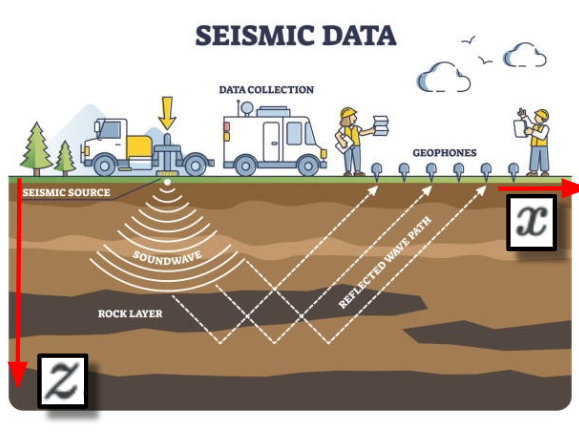
\includegraphics[width=0.48\linewidth]{figures/intro1.png}
    \hfill
    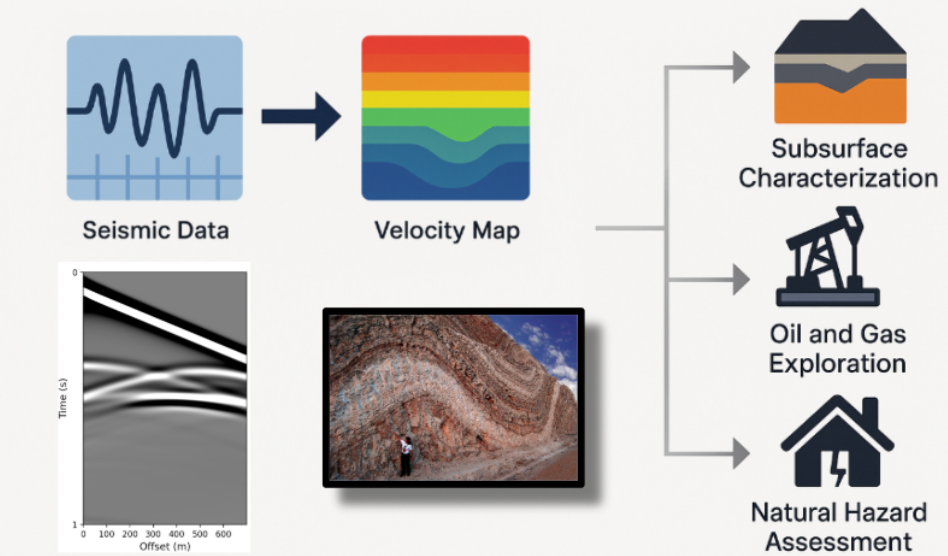
\includegraphics[width=0.48\linewidth]{figures/intro2.png}
    \caption{(Left) Surface-seismic acquisition. (Right) High-resolution velocity model inferred from recorded data.}
    \label{fig:intro}
\end{figure}

While underground receivers offer accurate data, they are costly and disruptive. Surface receivers are cheaper but introduce significant noise. Our work explores learning-based approaches to infer velocity maps from surface seismic data using various neural architectures.

We evaluate several models, including Fourier DeepONet, Residual UNet, InversionNet, VelocityGAN, 2D Fourier Neural Operator, Augmented Neural ODEs, and a PCA-based MLP. Fourier DeepONet achieved the best MAE of 59.54~m/s on our testing set, placing us \textbf{591st of 6446 entrants} in the Kaggle competition.

\paragraph{Contributions.}
Brief summary of our contributions (see Appendix for full breakdown):

\begin{itemize}[leftmargin=1.2em, itemsep=0.4em]
    \item \textbf{Fourier DeepONet:} Implemented spectral DeepONet with U-Net decoder; best performance on both datasets; evaluated noise robustness. [Girish]
    \item \textbf{Neural ODEs:} Built MLP and CNN-based Neural ODEs, including augmented variants. [Harini]
    \item \textbf{VelocityGAN \& InversionNet:} Reproduced and trained both baselines. VelocityGAN performed well; InversionNet overfit. [Girish]
    \item \textbf{Residual UNet:} Trained deeper UNet variant with skip connections. [Girish]
    \item \textbf{Fourier Neural Operator:} Adapted 2D FNO; stable but not state-of-the-art. [Yash]
    \item \textbf{PCA + MLP:} Designed a compact baseline combining PCA with MLP. Motivates future PCA-CNN variants. [Ryan]
\end{itemize}

\section{Related work} 
% \instructions{Related works [5\%]: Please review the related work in this area, state the challenges/limitations of the existing methods, and how does your proposed work will help address the prior limitations and/or advance the current state-of-the-art for this problem.}

The state-of-the-art paper for this problem is the Fourier DeepONet paper \cite{fdonet}, which showed that the Fourier DeepONet outperformed baselines such as InversionNet and VelocityGAN. However, this paper does not explore other potential architectures that could be used to solve the FWI problem. We decided to extend the results of this paper and adapt several models from papers shared in class to apply them to FWI, enabling direct performance comparisons with the Fourier DeepONet, InversionNet, and VelocityGAN. We implemented Augmented Neural ODEs \cite{anode} and the 2D Fourier Neural Operators \cite{fno}, and modified them for FWI.

In addition, PCA has previously been applied to geophysical waveform inversion problems, particularly in the context of classifying gas hydrates using an unsupervised neural network approach known as Self-Organizing Maps (SOM) \cite{jones2023waveform} . In that work, PCA was used to reduce the dimensionality of the input data before passing it to the SOM for clustering subsurface gas hydrate distributions \cite{jones2023waveform}. %, as illustrated in Figure~\ref{fig:related1}.

% commenting out this figure for now, as it seems pretty useless TBH

% \begin{figure}
%     \centering
%     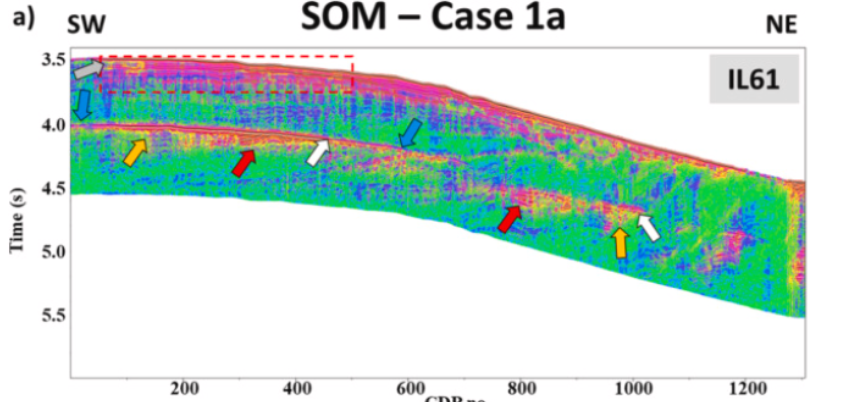
\includegraphics[width=0.5\linewidth]{figures/related1.png}
%     \caption{PCA-SOM approach for classifying gas hydrates underground \cite{jones2023waveform}.}
%     \label{fig:related1}
% \end{figure}

However, the task in \cite{jones2023waveform} is a classification problem, whereas our objective is to predict continuous velocity maps. Nevertheless, PCA remains an effective method for reducing dimensionality while retaining most of the variance in the dataset.

\section{Methodology}
% \instructions{Method/Approach [40\%]: this should be the main section of your report. Describe your approach, any equation and/or algorithm you developed to solve the problem. This part will be evaluated based on both scientific merit and technical depth.} \\

This section describes the different models we implemented along with their training strategies.

\subsection{Fourier DeepONet}

\begin{figure}
    \centering
    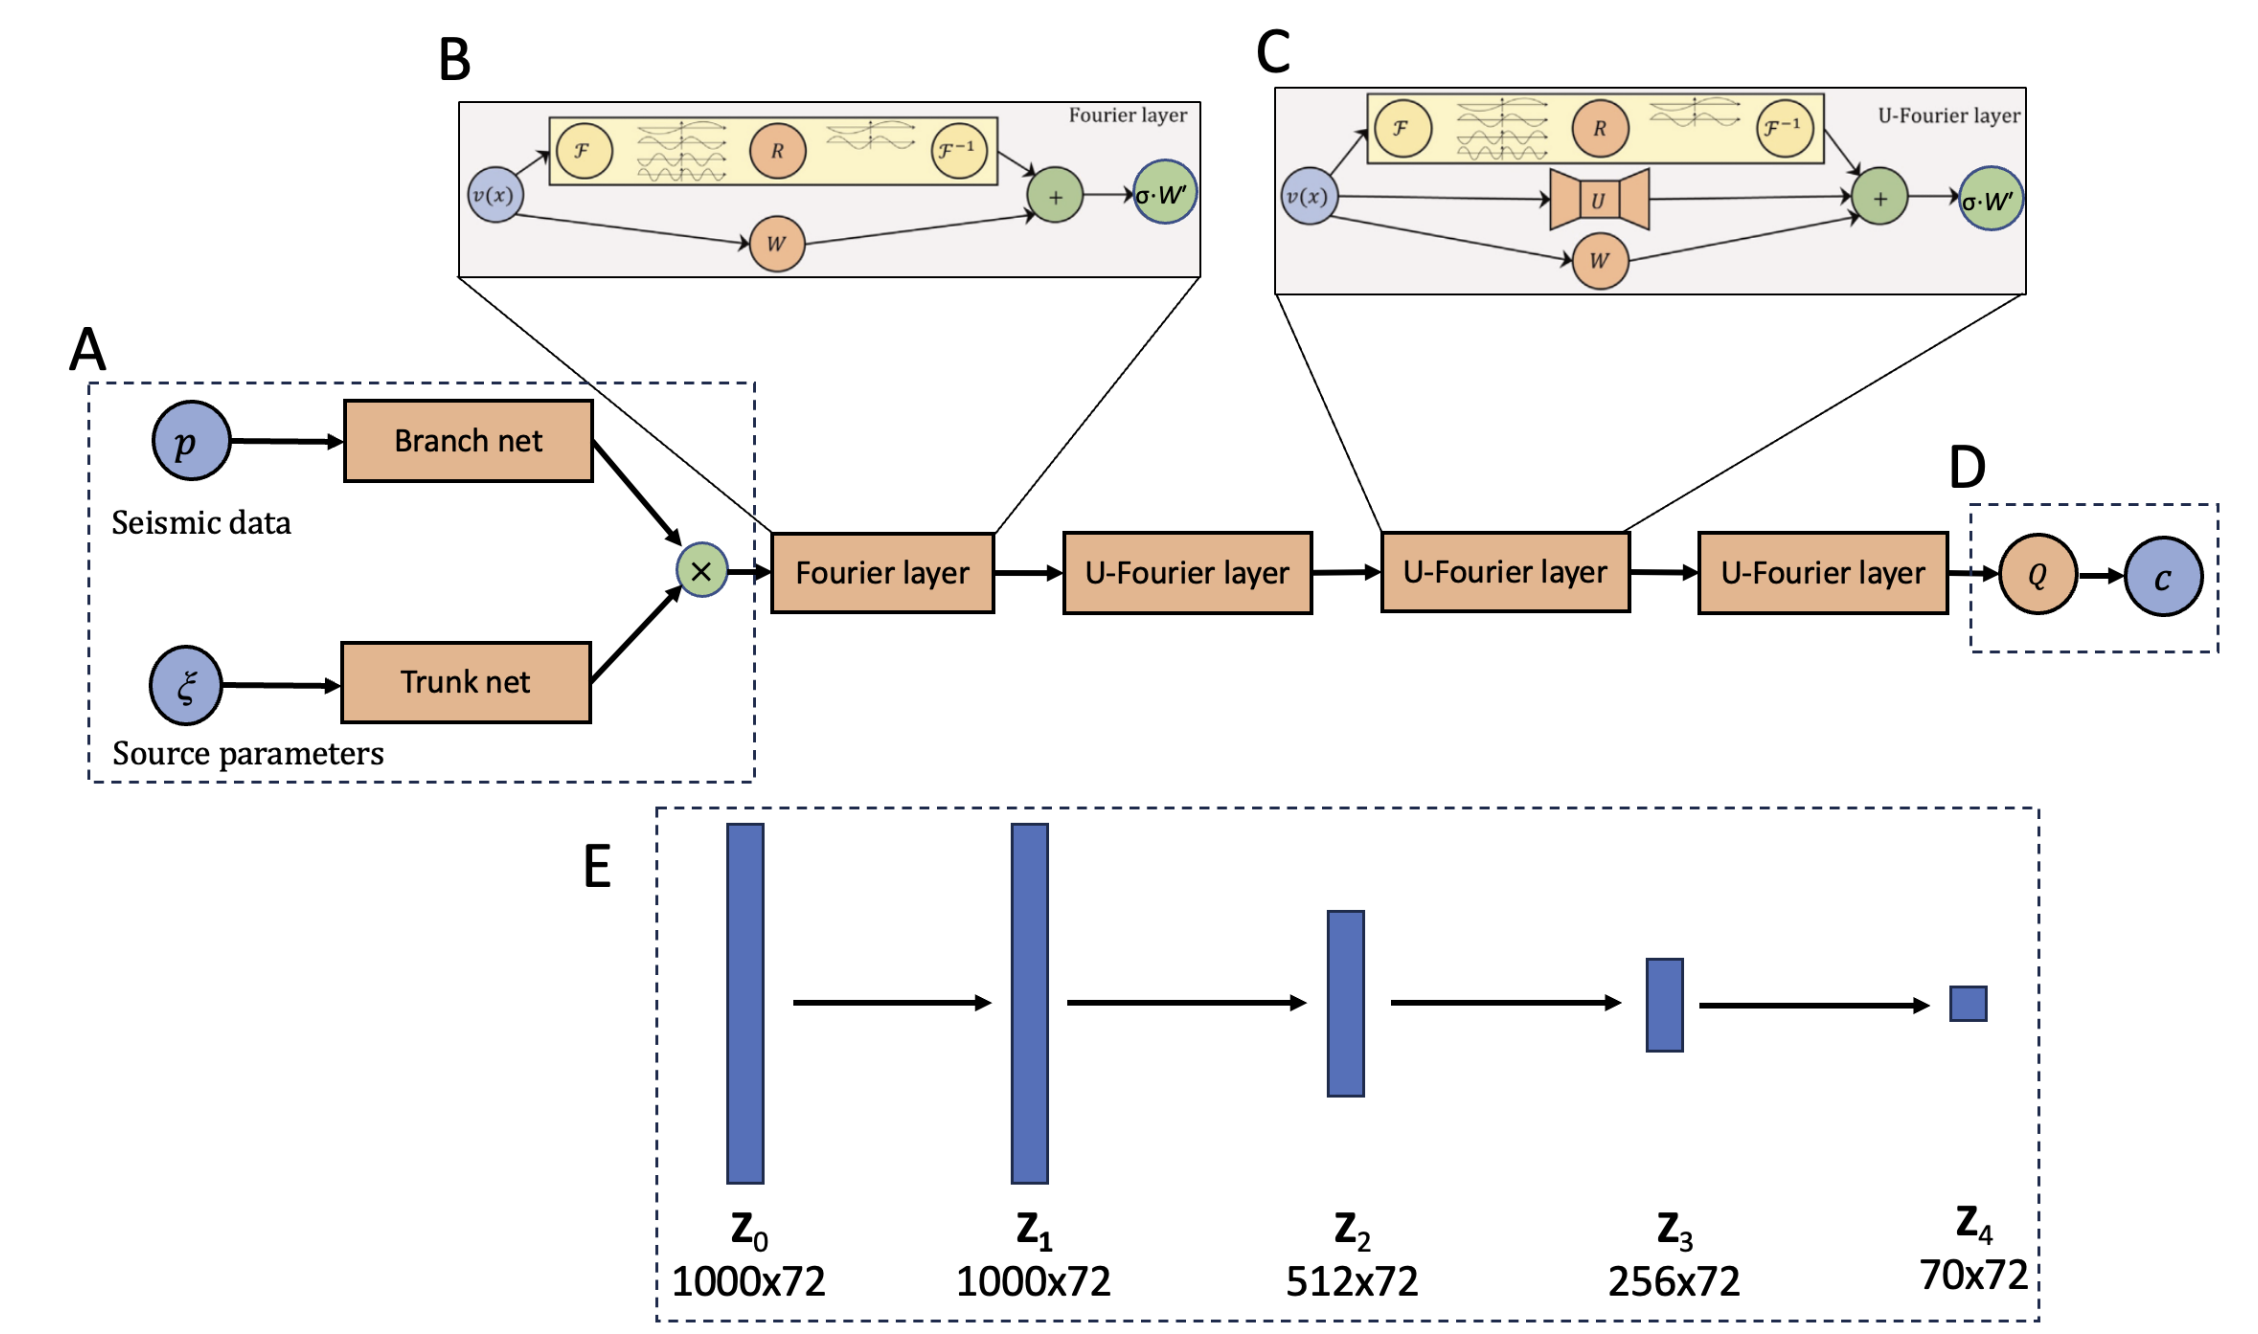
\includegraphics[width=0.8\linewidth]{figures/FDONet.png}
    \caption{\textbf{Fourier-DeepONet architecture.} 
    \textbf{(A)} Branch net and trunk net are two linear transformations lifting inputs to high dimensional space. Green circle represents the merger operation which denotes point-wise multiplication. 
    \textbf{(B)} Fourier layer, adapted from~\cite{li2020fourier}. 
    \textbf{(C)} U-Fourier layer, adapted from~\cite{wen2022u}. 
    \textbf{(D)} Projection layer $Q$. 
    \textbf{(E)} Shapes of outputs $\mathbf{z}_i$ in one channel, $i \in \{0,1,2,3,4\}$.
    \emph{Source}: \cite{fdonet}.}
    \label{fig:fdonet}
\end{figure}

Fourier DeepONet models the mapping from seismic observations \(u: \mathbb{R}^{5 \times 1000 \times 70}\) and a dummy parameter \(p\in\mathbb{R}\) to the velocity field \(v:\mathbb{R}^{70\times70}\). It consists of (i) \emph{Branch} network \(\mathcal{B}(u)\in \mathbb{R}^{w\times70\times70}\) implemented as a 2D linear lift, (ii) A \emph{Trunk} network \(\mathcal{T}(p)\in \mathbb{R}^{w\times1\times1}\), a simple MLP that conditions the operator. (iii) Element-wise multiplication \(\mathcal{B}(u)\odot\mathcal{T}(p)\), plus a learnable bias, serves as the input to the decoder.

The decoder consists of (i) Spectral convolution layers (\(\text{FourierConv}_\phi\)) that perform \(\hat v = \mathcal{F}^{-1}(R_\phi \cdot \mathcal{F}(v))\), processing data in Fourier space (ii) U-Fourier blocks that combine spectral convolutions with spatial skip connections via mini U-Nets and (iii) a projection layer \(Q\) that refines the feature maps.

Formally, if \(z_0 = \mathcal{B}(u)\odot\mathcal{T}(p)\), then for \(i=1,\dots,4\):
\[
z_i = \text{U-Fourier}\bigl(z_{i-1}\bigr),\quad
\hat{v} = Q(z_4),
\]
where each U-Fourier block is defined as
\[
\text{U-Fourier}(z) = \sigma\bigl(\text{Conv}_\text{Fourier}(z) + \text{Ublock}(z)\bigr).
\]
Finally, \(\hat v\) is linearly projected to a single-channel velocity field.

This architecture provides a unified latent representation (via branch–trunk conditioning) and achieves expressive approximation power through spectral convolution and multiscale U-blocks. Refer to Figure~\ref{fig:fdonet} for the overall structure.


\subsection{InversionNet and VelocityGAN}

\begin{figure}
    \centering
    \begin{subfigure}[b]{0.48\linewidth}
      \centering
      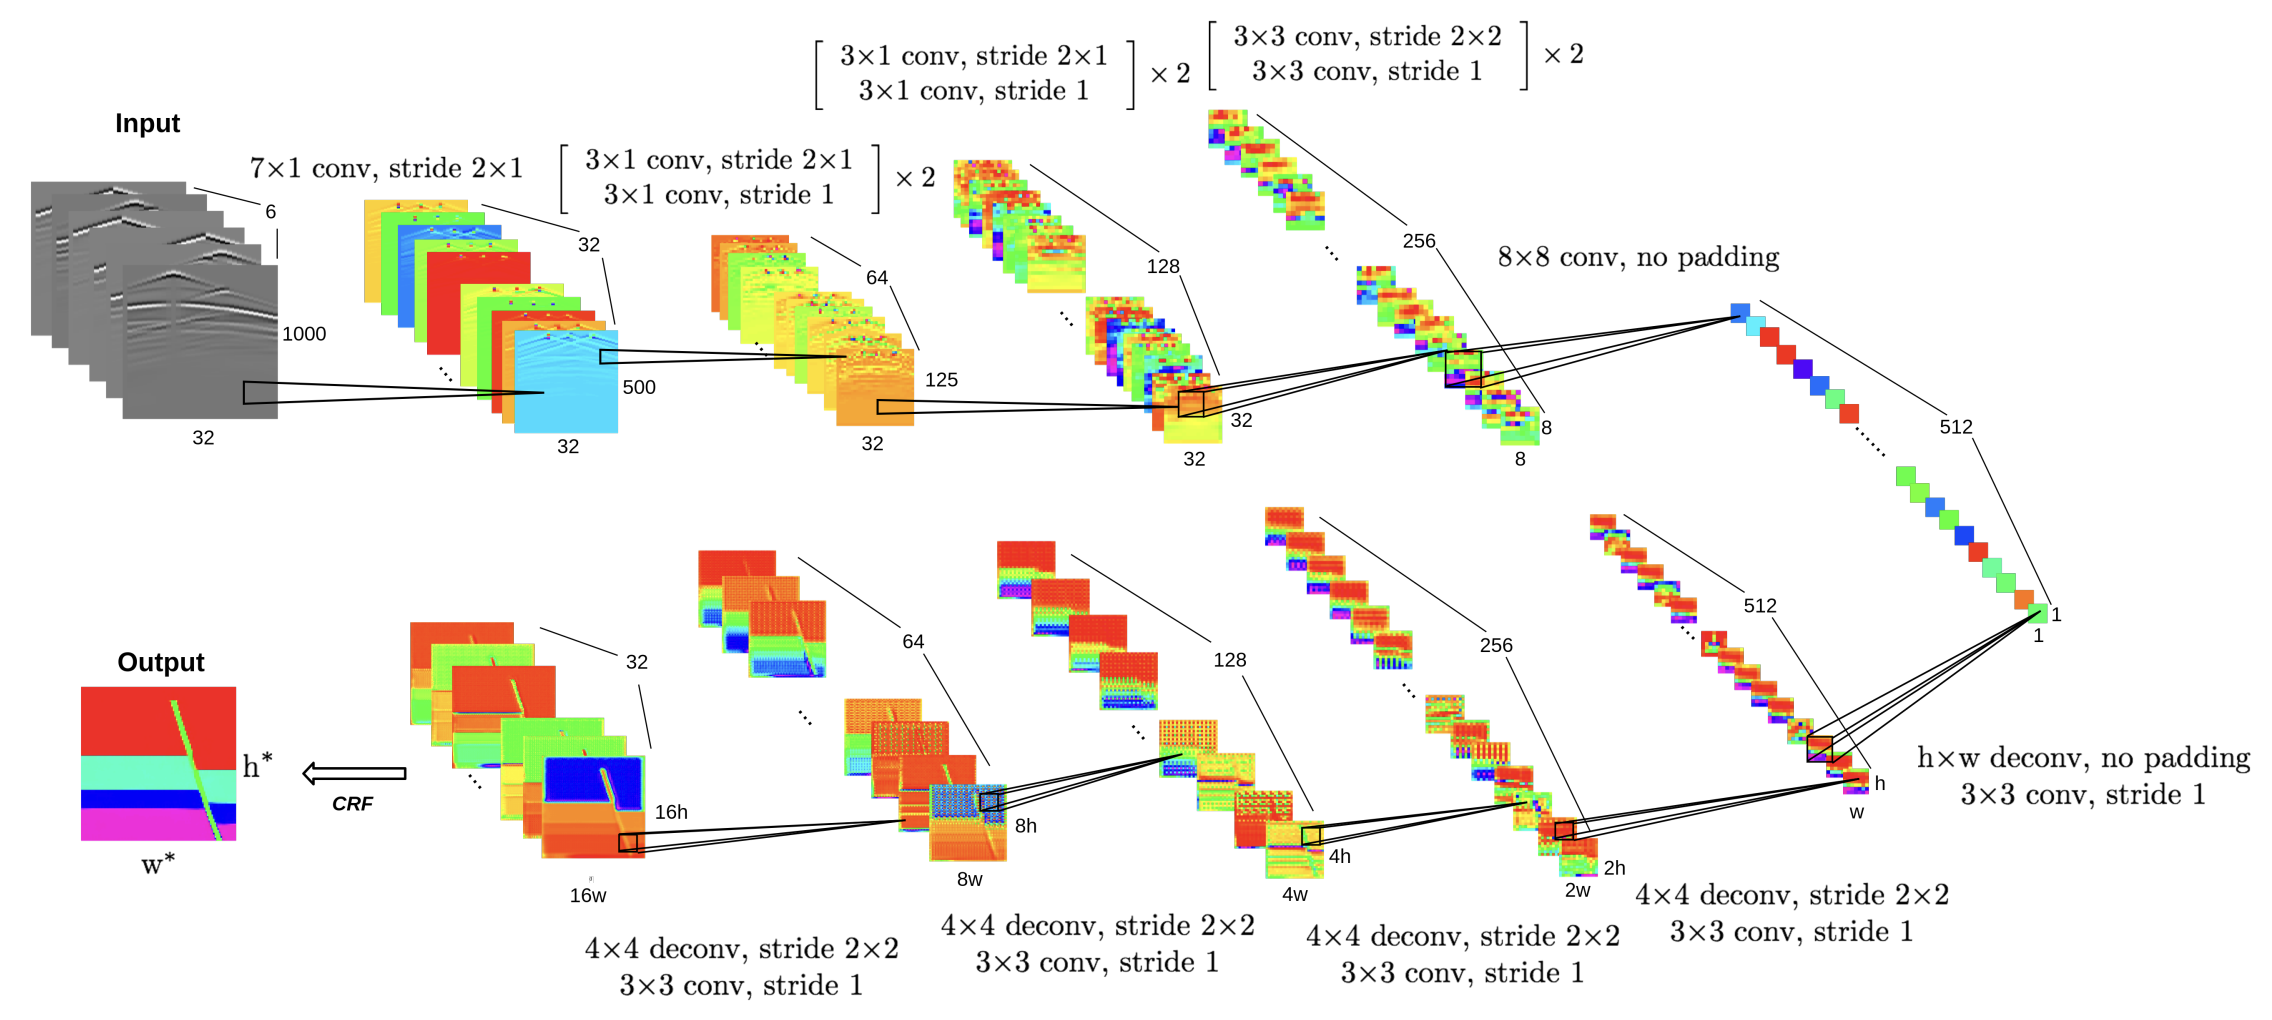
\includegraphics[width=\linewidth]{figures/InversionNet.png}
      \caption{InversionNet encoder–decoder.}
      \label{fig:inversionnet_sub}
    \end{subfigure}
    \hfill
    \begin{subfigure}[b]{0.48\linewidth}
      \centering
      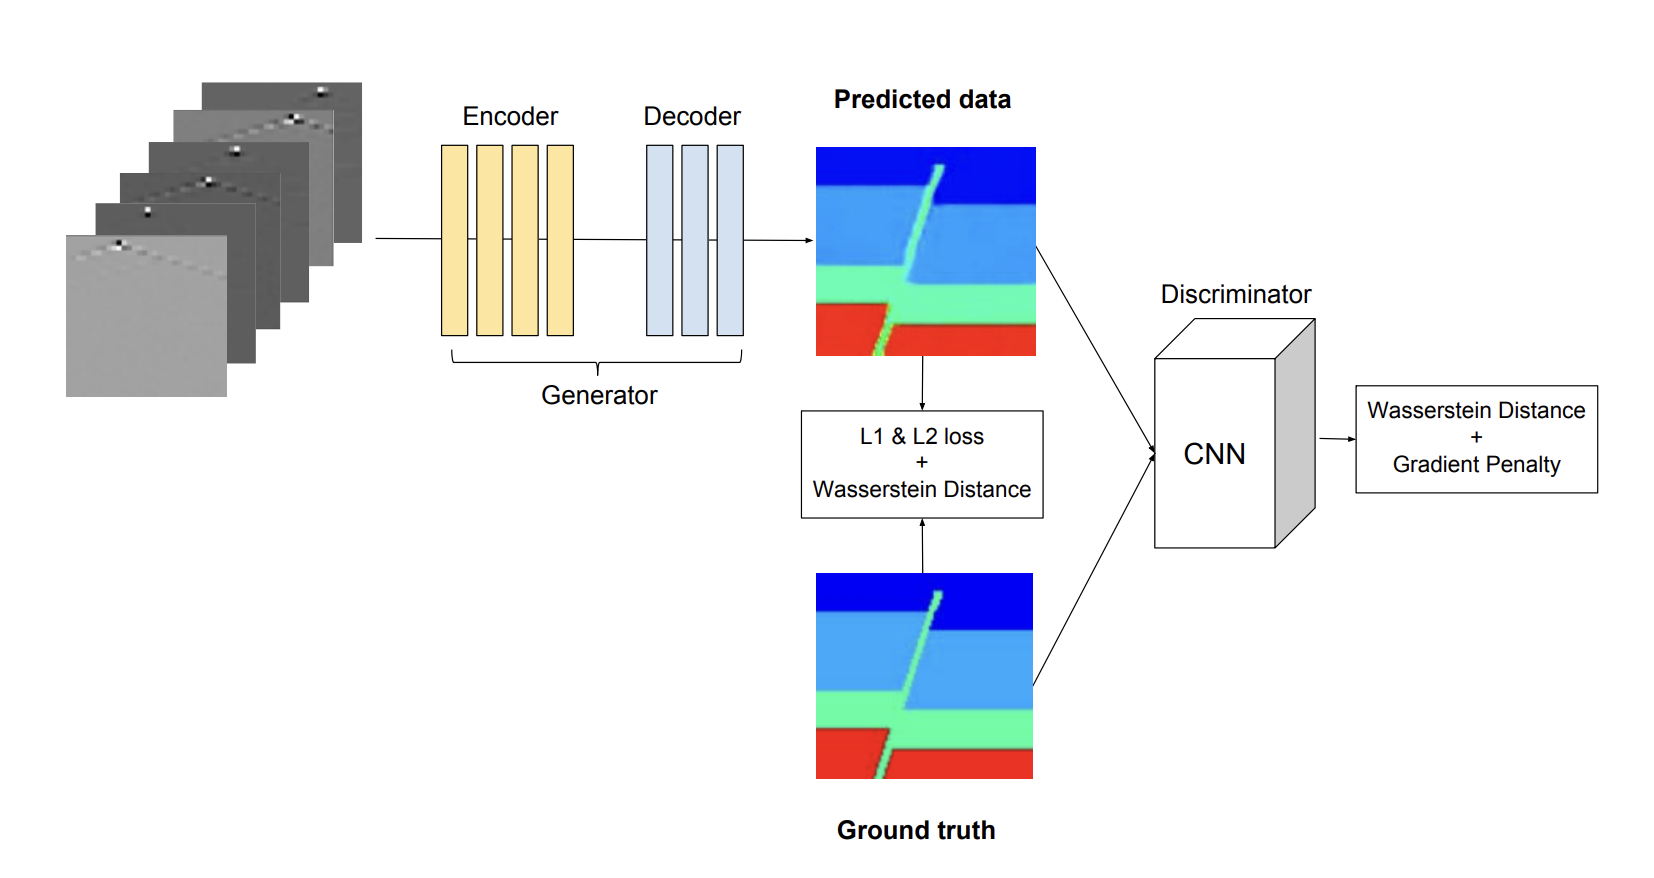
\includegraphics[width=\linewidth]{figures/VelocityGAN.png}
      \caption{VelocityGAN: InversionNet used as the generator.}
      \label{fig:velocitygan_sub}
    \end{subfigure}
    \caption{\textbf{(a)} InversionNet architecture: encoder compresses the input seismic cube $(B,5,1000,70)$ via successive conv/deconv layers, culminating in a tanh-activated $70\times70$ velocity map. \textbf{(b)} VelocityGAN setup: InversionNet serves as the generator $G$, and a patch-based CNN acts as discriminator $D$. The generator minimizes adversarial loss plus an $L_1$ term weighted by $\lambda$, while $D$ learns to distinguish real from generated maps.}
    \label{fig:inversion_velocitygan}
  \end{figure}
  
  Our implementation follows the LANL InversionNet design ~\cite{inversionnet, velocitygan}, employing a deep CNN encoder-decoder (Fig.~\ref{fig:inversionnet_sub}). The encoder maps the 3D seismic input to a compact bottleneck, and the decoder expands it to a $70\times70$ velocity map with Tanh activation in order to match the velocity range scaled to [-1,1]. In VelocityGAN, the same InversionNet functions as the generator $G$, paired with a CNN discriminator $D$ that outputs patch-wise real/fake scores (Fig.~\ref{fig:velocitygan_sub}).
  
  The generator is trained with a combined loss:
  \[
  \mathcal{L}_G = \mathrm{BCE}\bigl(D(G(s)),\,\mathbf{1}\bigr) + \lambda\,\lVert G(s) - v\rVert_1,
  \]
  where $\lambda = 100$ scales the MAE regularization, and the discriminator minimizes
  \[
  \mathcal{L}_D = \tfrac{1}{2}\bigl[\mathrm{BCE}(D(v),\,\mathbf{1}) + \mathrm{BCE}(D(G(s)),\,\mathbf{0})\bigr].
  \]
  This adversarial setup encourages the generator to produce velocity maps that are both accurate and structurally realistic.  



\subsection{Residual UNet}

\begin{figure}
    \centering
    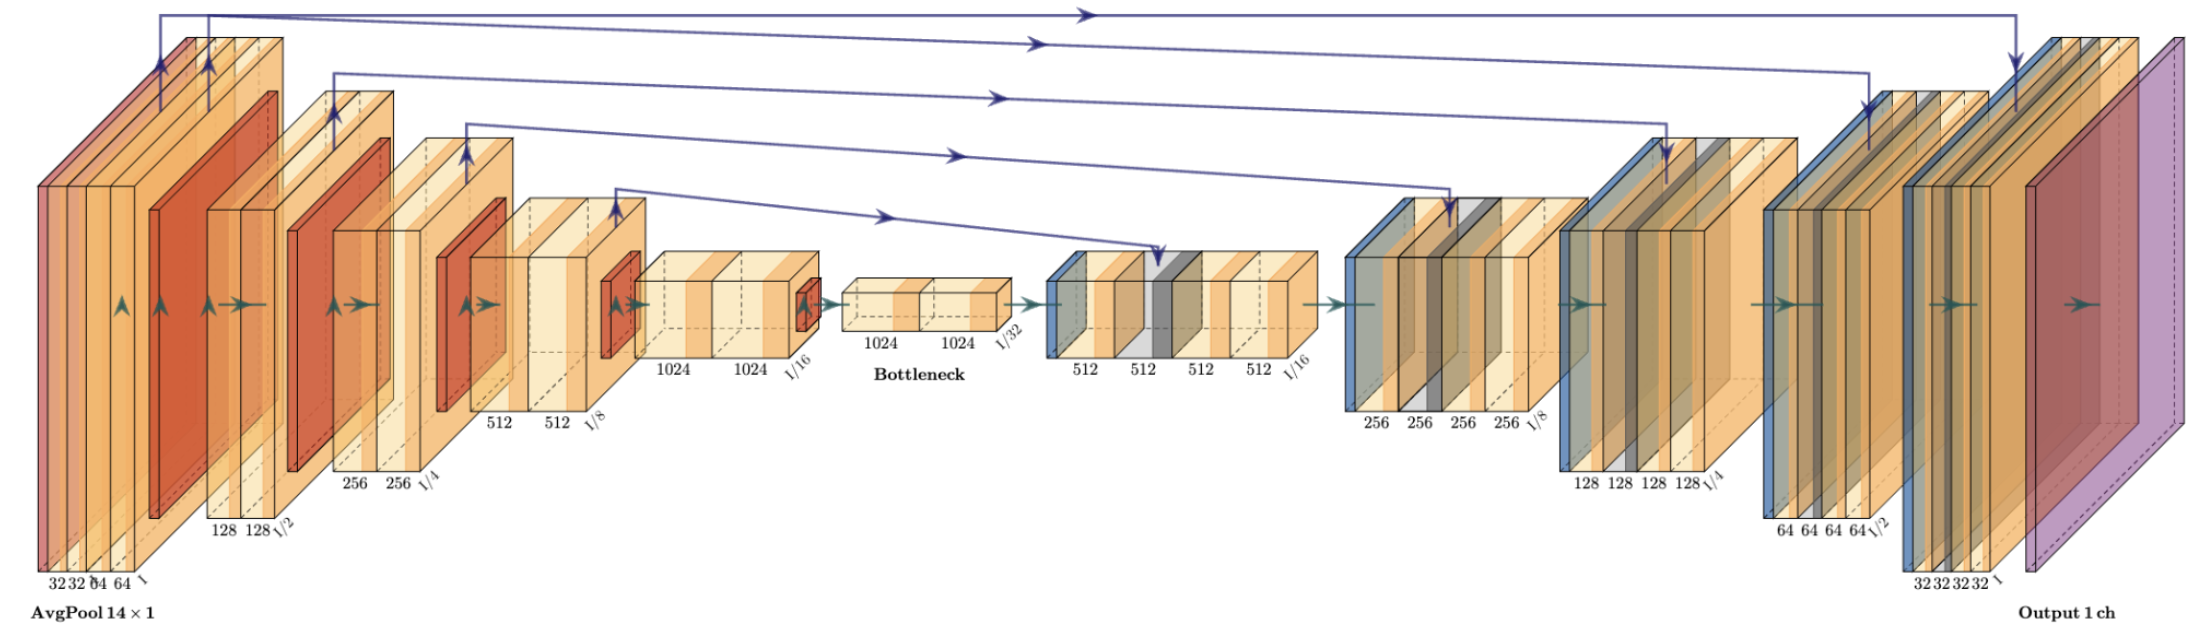
\includegraphics[width=0.8\linewidth]{figures/ResidualUNet.png}
    \caption{Residual UNet architecture for seismic-to-velocity inversion. The network uses an encoder to compress the input seismic cube into latent features and a decoder with symmetric up-sampling paths that leverage skip connections. Residual blocks ensure stable gradient flow and enable training of deeper architectures.}
    \label{fig:residual_unet}
\end{figure}

Residual UNet adapts the widely used U-Net~\cite{ronneberger2015u} by integrating residual connections from ResNet~\cite{he2016deep} into each convolutional block. As shown in Figure~\ref{fig:residual_unet}, the network comprises a down-sampling path that applies multiple \emph{ResidualDoubleConv} modules to encode the 5×1000×70 seismic input into a lower-dimensional latent representation. In the up-sampling path, each decoder block receives concatenated features from its encoder counterpart via skip connections, followed by residual up-convolution to reconstruct a 70×70 velocity map.

Formally, each residual block computes:
\[
\mathbf{y} = \sigma\bigl(\mathrm{BN}(W_2 * \sigma(\mathrm{BN}(W_1 * \mathbf{x}))) + \mathcal{S}(\mathbf{x})\bigr),
\]
where \( * \) denotes convolution, \(\mathrm{BN}\) denotes batch normalization, \(\sigma\) is ReLU, and \(\mathcal{S}\) is either identity or a learned linear shortcut. These shortcuts enable smoother gradient propagation through the network.

Several top-performing competitors in the Kaggle competition employ similar architectures, primarily due to the network's ability to capture fine structural details while maintaining global context.

\subsection{Neural ODE}
\begin{figure}
    \centering
    \begin{subfigure}[b]{0.47\linewidth}
        \centering
        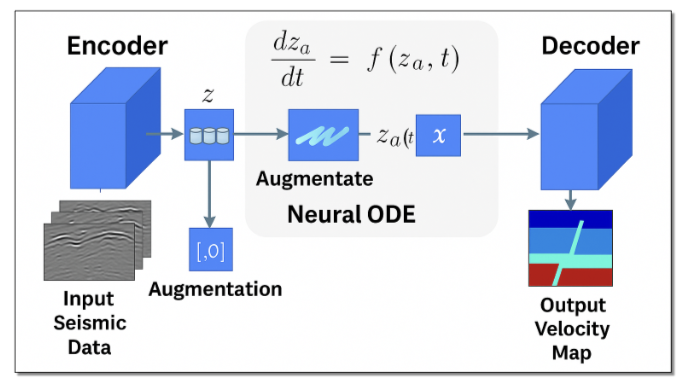
\includegraphics[width=\linewidth]{figures/neuralode_structure.png}
        \caption{General structure}
    \end{subfigure}
    \hfill
    \begin{subfigure}[b]{0.47\linewidth}
        \centering
        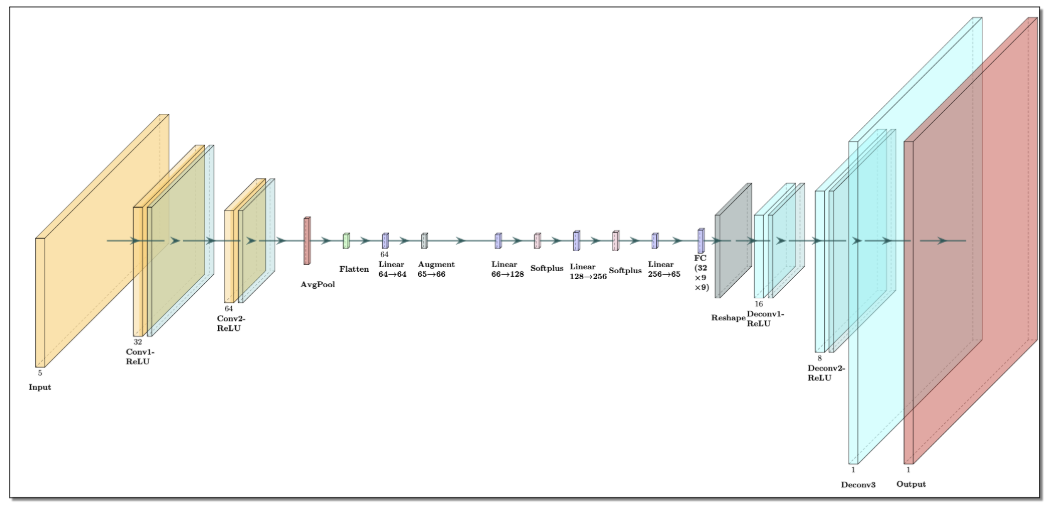
\includegraphics[width=\linewidth]{figures/augmented_neuralode.png}
        \caption{Augmented MLP base}
    \end{subfigure}
    \caption{Augmented Neural ODE architectures. (a) shows the general structure, where input seismic data is encoded, augmented, solved via ODE integration, and decoded to produce the velocity map. (b) shows the specific Augmented Neural ODE model using an MLP base function.}
    \label{fig:neuralode-merged}
\end{figure}

One of the models chosen to experiment with was the Neural ODE as learned in the course. Neural ODEs are differential equation solvers, with the solver essentially being a black box. The model can be implemented by using the \texttt{torchdiffeq} package in Python and the function \texttt{odeint} from this package. The structure of this model was a convolutional encoder, a three-layer MLP as the base function, and a decoder to shape the output as a 70×70 tensor to compare against the ground truth. 

Two different Augmented Neural ODEs were also created. One model had the same MLP as a base function and the other had a simple convolutional network as its base. Both models had an augmented dimension of 1. Augmented Neural ODEs were chosen because the augmented dimension helps in cases where an extra dimension is needed so that trajectories do not intersect.

As illustrated in \textbf{Figure~\ref{fig:neuralode-merged}}, the input seismic data is passed into an encoder and then augmented. This augmented data is passed into the differential equation solver and then decoded into the output velocity map. Subfigure (b) in particular shows the more specific structure of the Augmented Neural ODE with an MLP base.


\subsection{2-Dimensional Fourier Neural Operator}

Another model we tried was an adaptation of the Fourier Neural Operator \cite{fno} we learned about in class and experimented with in the homework. Since our input seismic data had both spatial and time dimensions and was required to produce a 2-dimensional velocity map, we adapted the Fourier Neural Operator such that it used 2D Fast Fourier Transforms in the spectral convolution.

The architecture shown in \textbf{Figure \ref{fig:fno-2d}} starts off with a 2D convolution-based encoder that takes the seismic data and encodes it into 70×70 arrays used to learn the velocity map. It then average-pools the data to extract representative features from the original data stream. This is followed by grid concatenation; Fourier neural operators are fairly sensitive to grid resolution. The grid was chosen to have a step size of 0.2 to regularize the spatial steps taken by the data. Post concatenation, the data was passed through four series of spectral convolutions that perform Fourier transforms on the data, carry out weighted multiplications, and finally apply an inverse transform to prepare the data for the next block. \textbf{Figure \ref{fig:fno-2d}}(b) shows the internal structure of a single spectral convolution block. This was implemented with skip connections such that original data was weighted (through separate convolution layers) and added to the spectral outputs. Lastly, the model performs a decoding and projection to produce the velocity map predictions.

\begin{figure}
    \centering
    \begin{subfigure}[b]{0.6\linewidth}
        \centering
        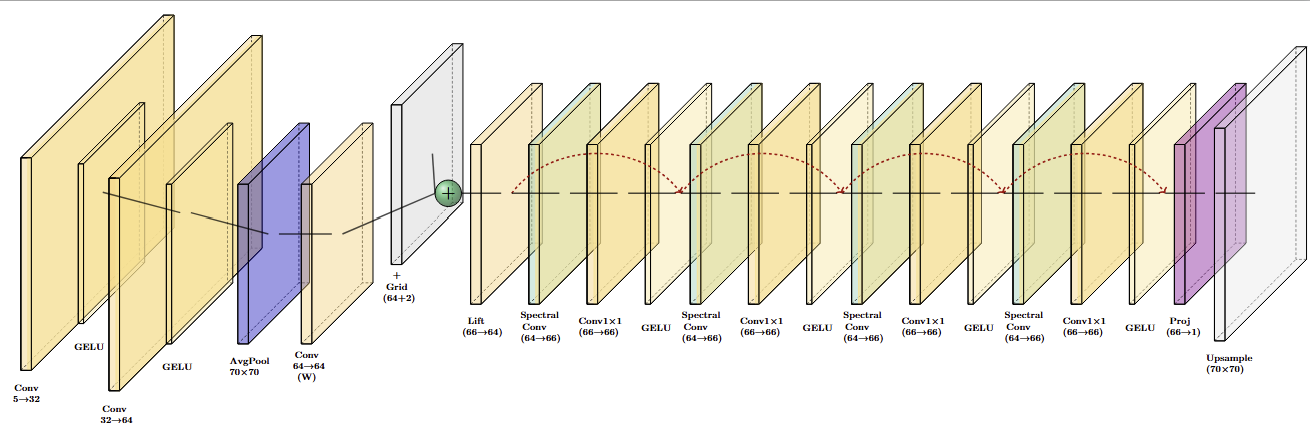
\includegraphics[width=\linewidth]{figures/FNO2D.png}
        \caption{2D Fourier Neural Operator}
    \end{subfigure}
    \hfill
    \begin{subfigure}[b]{0.3\linewidth}
        \centering
        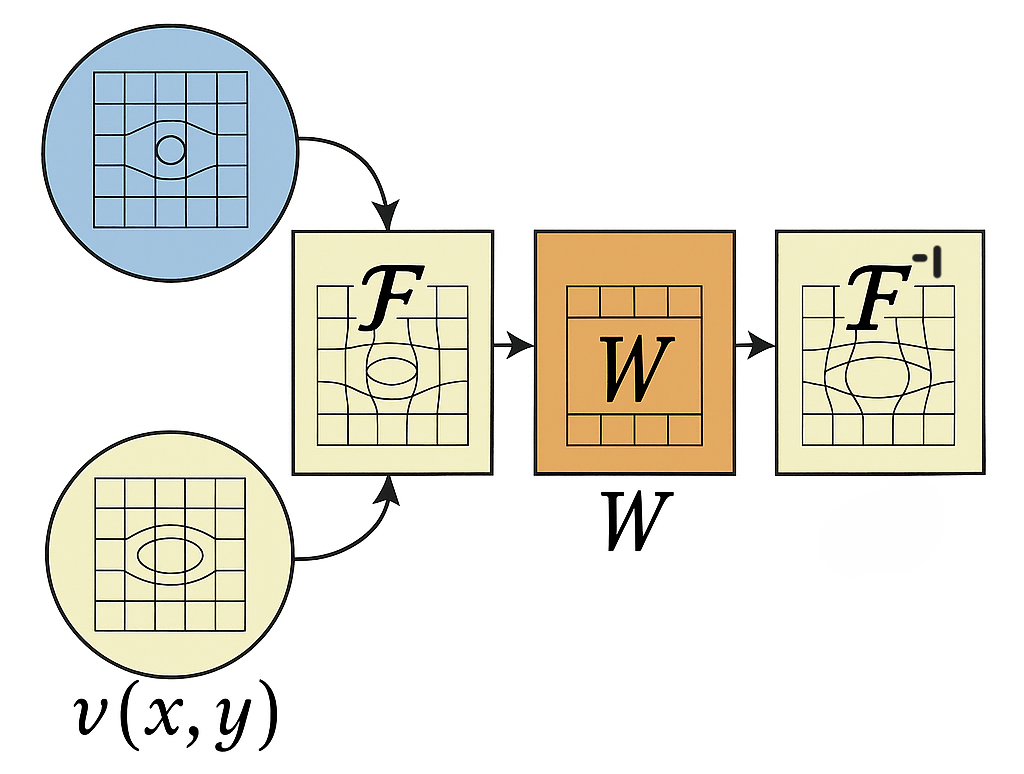
\includegraphics[width=\linewidth]{figures/spectralconv2d.png}
        \caption{Spectral Convolution Block}
    \end{subfigure}
    \caption{(a) Full 2D Fourier Neural Operator architecture used in our experiments. (b) Internal schematic of the spectral convolution block.}
    \label{fig:fno-2d}
\end{figure}

\subsection{Principal Component Analysis (PCA) along with MLP} 

To perform Principal Component Analysis (PCA), one must first normalize the data. The most common method of doing so is via Z-score normalization $(x - \mu)/\sigma$, where $\mu$ is the mean, $\sigma$ is the standard deviation, and $x$ is the data point. The reason for normalizing the data is so that features with inherently larger magnitudes do not overshadow those with smaller magnitudes. For example, the number of molecules in a human is several orders of magnitude larger than human height in inches.

After normalization, we perform PCA by calculating the eigenvectors of the covariance matrix, which represent the principal components. Each principal component (PC) is an eigenvector that captures a direction of maximum variance in the data and is orthogonal to the previous PCs. The weights associated with each PC are known as loading scores and indicate how much a PC accounts for variability in the dataset. The PCs now act as the new dependent variables instead of our original features.

\begin{figure}
    \centering
    \begin{subfigure}[b]{0.45\linewidth}
        \centering
        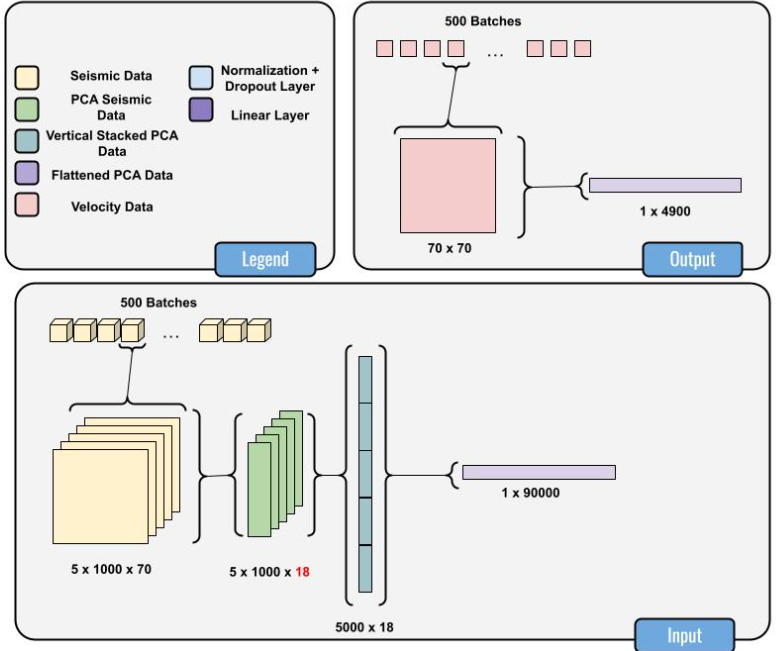
\includegraphics[width=\linewidth]{figures/PCA1.png}
        \caption{PCA Data Preparation}
    \end{subfigure}
    \hfill
    \begin{subfigure}[b]{0.45\linewidth}
        \centering
        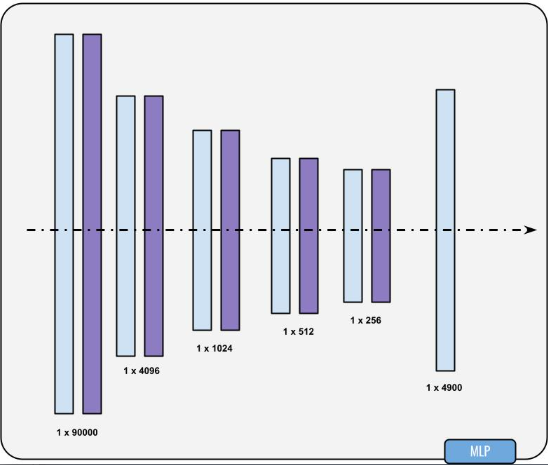
\includegraphics[width=\linewidth]{figures/PCA2.png}
        \caption{PCA-MLP Architecture}
    \end{subfigure}
    \caption{(a) Seismic waveform data reshaped and reduced via PCA. (b) MLP model applied to PCA-transformed data.}
    \label{fig:pca}
\end{figure}

PCA is performed on the seismic waveform dataset by first taking a single batch with dimensions $5 \times 1000 \times 70$. We then extract each source individually, resulting in a $1000 \times 70$ matrix where each column represents a given receiver. Because of the large number of receivers, we aim to reduce this dimension since many may provide redundant data. We reduce this from 70 receivers to 18 principal components. Empirical testing showed that 18 PCs consistently captured about 95\% of the variance for each source. To allow consistent stacking of all sources, we use a fixed number of PCs rather than selecting the minimum needed per source. This results in a $5000 \times 18$ matrix, which is flattened into a single feature vector per batch. All batches are stacked to form the full dataset, which serves as input to the model.

The transformed data is then passed through a multi-layer perceptron (MLP), with normalization and dropout applied to each layer.

\section{Experiments}
% \instructions{Results [30\%]: present your results and provide sufficient discussions of the results. 1) Describe what dataset is being used, details in data processing, train-test data split, and hyperparameter choices in your model etc. Provide the sufficient details such that if a reader would like to reproduce your results, they have enough information to do it. 2) Include figures and/or tables showing the quantitative and qualitative performance of your method; 3) Comparison to necessary baseline methods and comparison to your proposed method.} 

\subsection{Dataset and Data Processing}\label{subsec:data}
\textsc{OpenFWI} is a public, 622\,GB benchmark that gathers multi\-fold synthetic seismic‐to‐velocity pairs generated with finite‐difference forward modelling over a variety of 2-D geological scenarios (e.g.\ \emph{FlatVel}, \emph{CurveVel}, \emph{FlatFault}, \emph{CurveFault}, \emph{Style}) \cite{openfwi2021,openfwi2023}.  Each sample consists of a tensor of raw pressure gathers $\mathbf{s}\!\in\!\mathbb{R}^{5\times1000\times70}$ (five sources, 1000 time steps, 70 receivers) and its corresponding velocity map $v\!\in\!\mathbb{R}^{1\times70\times70}$.  
For rapid prototyping we curate a \emph{small subset} composed of one 500-sample batch from the categories \texttt{CurveFault\_A}, \texttt{CurveVel\_A}, \texttt{FlatFault\_A}, and \texttt{Style\_A} (2 000 samples in total).  
After min–max normalization of velocity ($1500$–$4500$\,m/s) and $\log$–amplitude scaling of gathers, the subset is randomly divided 70\% / 20\% / 10\% into training, validation, and test partitions.  
The best architecture found on this subset is subsequently trained on the \emph{full} OpenFWI corpus and submitted to the Kaggle “Geophysical Waveform Inversion’’ leaderboard.

\subsection{Evaluation metrics}\label{subsec:metrics}
Model outputs $\hat{v}$ are compared with ground-truth velocity maps $v$ using four complementary criteria that jointly capture absolute error, outlier sensitivity, structural fidelity, and scale\,/\,magnitude awareness using the metrics summarized in Table \ref{tab:metrics}.

\begin{table}
    \centering
    \renewcommand{\arraystretch}{1.4}
    \begin{tabular}{@{}p{1cm} p{8cm} c@{}}
    \toprule
    \textbf{Metric} & \textbf{Description} & \textbf{Formula} \\
    \midrule
    MAE & Measures average absolute difference between predicted and ground truth values. Also the primary metric used in the Kaggle competition. & 
    $\displaystyle \frac{1}{N} \sum_{i=1}^{N} |y_i - \hat{y}_i|$ \\
    \addlinespace
    RMSE & Penalizes large errors more than MAE; helpful for evaluating overall accuracy. &
    $\displaystyle \sqrt{ \frac{1}{N} \sum_{i=1}^{N} (y_i - \hat{y}_i)^2 }$ \\
    \addlinespace
    SSIM & Captures perceptual similarity by comparing luminance, contrast, and structure. Useful for assessing structural fidelity. &
    $\displaystyle \frac{(2\mu_x \mu_y + C_1)(2\sigma_{xy} + C_2)}{(\mu_x^2 + \mu_y^2 + C_1)(\sigma_x^2 + \sigma_y^2 + C_2)}$ \\
    \addlinespace
    Relative $\ell_2$ Error & Measures the relative difference scaled by the ground truth magnitude. Provides a normalized global error measure. &
    $\displaystyle \frac{ \| y - \hat{y} \|_2 }{ \| y \|_2 }$ \\
    \bottomrule
    \vspace{0.1em}
    \end{tabular}
    \caption{Evaluation metrics used to quantify model performance on velocity map prediction. In the SSIM formula, $\mu_x$ and $\mu_y$ denote the local means of the predicted and ground truth images respectively, $\sigma_x^2$ and $\sigma_y^2$ are their local variances, $\sigma_{xy}$ is the local covariance, and $C_1$, $C_2$ are small constants that stabilize the division to avoid numerical instability.}
    \label{tab:metrics}
\end{table}

All metrics are reported on the held-out test split of the subset. For the best-performing model, we also report the MAE on the full OpenFWI dataset, which is used to rank submissions in the Kaggle competition.

\subsection{Hyperparameters and Training}

All models were trained on a single GPU (provided on DSMLP) with mixed‐precision (\texttt{torch.cuda.amp}) and the same 70 / 20 / 10 train-val-test split described earlier. Core hyper-parameters were selected with a 40–trial Optuna Bayesian search per model, using validation MAE as the objective.  Table~\ref{tab:hparams} summarizes the final settings.

\begin{table}
    \centering
    \footnotesize
    \renewcommand\arraystretch{1.05}
    \newcolumntype{Y}{>{\raggedright\arraybackslash}X}
    \begin{tabularx}{\linewidth}{@{}l c c c c c Y@{}}
    \toprule
    \textbf{Model} & \textbf{Opt.} & \textbf{LR} & \textbf{B} & \textbf{Ep.} & \textbf{Loss} & \textbf{Scheduler / key architectural settings} \\
    \midrule
    Fourier DeepONet      & Adam & $1\!\times\!10^{-3}$ & 4  & 100 & $\ell_1$ &
    \makecell[l]{width 64,\; modes $20\!\times\!20$} \\
    
    InversionNet          & Adam & $1\!\times\!10^{-3}$ & 8  & 100 & $\ell_1$ &
    --- \\
    
    VelocityGAN (G)       & Adam & $2\!\times\!10^{-4}$ & 8  & 50  & $\text{BCE}+\lambda\ell_1$ &
    $\lambda\!=\!100,\;\beta=(0.5,0.999)$ \\
    
    VelocityGAN (D)       & Adam & $2\!\times\!10^{-4}$ & 8  & 50  & BCE &
    $\beta=(0.5,0.999)$ \\
    
    Residual UNet         & Adam & $1\!\times\!10^{-3}$ & 8  & 100 & $\ell_1$ &
    depth 5,\; init‐feat 32 \\
    
    2-D FNO               & Adam & $5\!\times\!10^{-3}$ & 4  & 250 & $\ell_1$ &
    StepLR$\,(\!\times0.5\!/\!75$ep), modes $32\!\times\!32$, width 64, layers 4 \\
    
    Neural ODE (MLP)      & Adam & $1\!\times\!10^{-3}$ & 8  & 50  & $\ell_1$ &
    StepLR$\,(\!\times0.5\!/\!10$ep), tol $10^{-3}$, max 100 steps \\
    
    Aug.\ ODE (MLP)       & Adam & $1\!\times\!10^{-3}$ & 8  & 50  & $\ell_1$ &
    as above,\; aug.\ dim 1 \\
    
    Aug.\ ODE (CNN)       & Adam & $1\!\times\!10^{-3}$ & 8  & 50  & $\ell_1$ &
    CNN base,\; aug.\ dim 1 \\
    
    PCA\,+\,MLP           & Adam & $1.5\!\times\!10^{-1}$ & 16 & 100 & MSE &
    StepLR$\,(\!\times0.5\!/\!15$ep), hidden [2048,512,128], drop 0.05 \\
    \bottomrule
    \end{tabularx}
    \caption{Final hyper-parameters.  LR = learning rate, B = batch size, Ep. = epochs.}
    \label{tab:hparams}
\end{table}

\paragraph{Training protocol.}  
Unless otherwise stated, gradients were unclipped and weight decay was set to
$10^{-4}$ for operator-style models (FNO, ODE variants) and omitted elsewhere.
Mini‐batches were shuffled each epoch and early stopping with a
patience of 15 epochs was employed during the Optuna search; the best
checkpoint was then retrained from scratch with the hyper-parameters shown
above.  All reported test scores (Table~\ref{tab:quant}) correspond to these
re-trained models.

\subsection{Quantitative Results}

Table \ref{tab:quant} reports validation MAE (used for early stopping) and four
test-set metrics for all nine models.  Lower is better except for SSIM, where
higher indicates greater structural fidelity.

\begin{table}[H]
\centering
\small
\renewcommand{\arraystretch}{1.15}
\setlength{\tabcolsep}{5pt}
\begin{tabular}{@{}lccccc@{}}
\toprule
\textbf{Model} & \textbf{Val.\ MAE} $\downarrow$ & \textbf{Test MAE} $\downarrow$ & \textbf{RMSE} $\downarrow$ & \textbf{SSIM} $\uparrow$ & \textbf{Rel.\ $L_2$} $\downarrow$ \\
\midrule
Fourier DeepONet                & 59.5 & \textbf{71.4} & \textbf{76.3} & \textbf{0.916} & \textbf{0.029} \\
VelocityGAN                     & \textbf{52.3} & 72.4 & 114.7 & 0.904 & 0.044 \\
InversionNet                    & 68.1 & 82.5 & 135.6 & 0.634 & 0.052 \\
Residual UNet                   & 68.4 & 72.4 & 146.4 & 0.903 & 0.049 \\
Fourier Neural Operator (2-D)   & 124.2 & 106.9 & 166.7 & 0.727 & 0.056 \\
Neural ODE (MLP)                & 468.2 & 471.5 & 595.0 & 0.879 & 0.199 \\
Aug.\ Neural ODE (MLP)          & 468.0 & 471.4 & 595.2 & 0.876 & 0.199 \\
Aug.\ Neural ODE (CNN)          & 468.0 & 471.4 & 595.2 & 0.876 & 0.199 \\
PCA\,+\,MLP                     & 311.8 & 308.0 & 430.0 & 0.707 & 0.151 \\
\bottomrule
\end{tabular}
\caption{Performance on the held-out test split (\(N\!=\!200\)).
Best value in each column is \textbf{bold}.}
\label{tab:quant}
\end{table}

\subsection{Qualitative Results}

Figure \ref{fig:qualitative_results} shows qualitative results for the best-performing model (Fourier DeepONet) and the baseline InversionNet. The predicted velocity maps exhibit high structural fidelity, with the Fourier DeepONet capturing fine details and long-range correlations better than the other models.

\begin{figure}
    \centering
    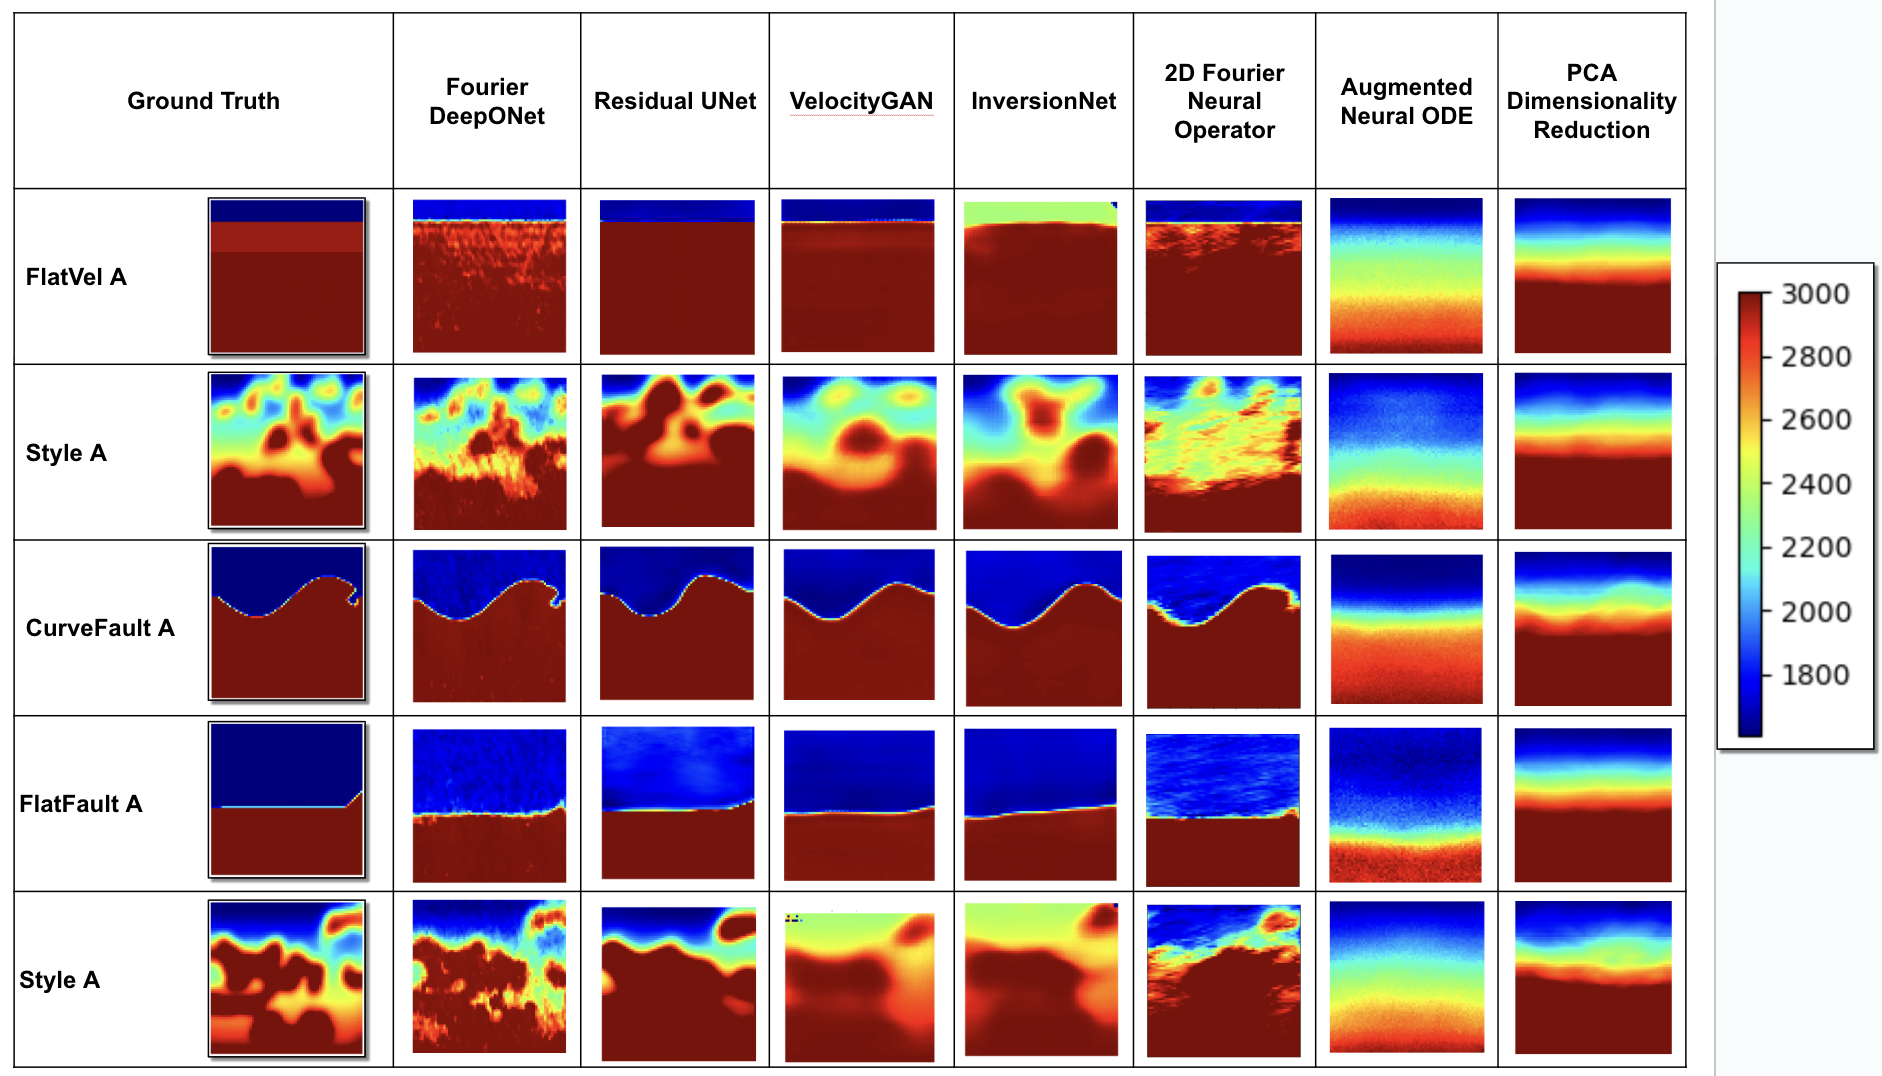
\includegraphics[width=\linewidth]{figures/qualitative_results.png}
    \caption{Qualitative comparison of predicted velocity maps from different models against the ground truth. Each row corresponds to a different sample in the testing set, with the first column showing the ground truth velocity map. The subsequent columns show the predictions from each model. The colorbar indicates the velocity scale in m/s. The Fourier DeepONet predictions closely match the ground truth, while other models exhibit varying degrees of deviation.}
    \label{fig:qualitative_results}
\end{figure}

\subsection{Ablation Studies}

\subsubsection{2D Fourier Neural Operator Ablation}
\textcolor{blue}{\textbf{TODO:} Yash will add experiments and results for the 2D Fourier Neural Operator ablation.}

\subsubsection{Neural ODE and Augmented Neural ODE Ablation}
For the standard Neural ODE, one of the hyperparameters experimented with was the hidden dimension that was used between the encoder, solver, and decoder. Originally, 128 was used but this made the model too complex and increased training time, so it was reduced to 64. Another hyperparameter was the learning rate, which was originally at $1 \times 10^{-4}$ but was changed to $1 \times 10^{-3}$ because the smaller learning rate did not improve accuracy significantly. Batch size was reduced from 32 to 8 because of CUDA memory errors. Lastly, tolerance was chosen to be $1 \times 10^{-3}$ and maximum number of steps was 100 for a quicker convergence for the differential equation solver. For the Augmented Neural ODE with the MLP base, the same hyperparameters were used. An augmented dimension of one was chosen because the model learned without augmentation, so an additional dimension was added as an experiment to see if it would improve learning. For the Augmented Neural ODE with a CNN base, the learning rate was $3\times 10^{-4}$, because $1 \times 10^{-4}$ had a slower convergence and $1 \times 10^{-3}$ was leading to instability. A weight decay of $5 \times 10^{-5}$ was also chosen for the optimizer. After hyper-parameter experimentation and selection, the metrics computed were similar amongst all three models.

\subsection{Discussion and Model Comparison}
Fourier DeepONet dominates every error metric, confirming that its
spectral-operator design excels at capturing long-range, multi-scale
dependencies present in seismic data.
VelocityGAN achieves the lowest \emph{validation} MAE, but is narrowly
outperformed by DeepONet on the test set as it has the tendency to
slightly over-fit small training corpora.
Residual UNet matches GAN-level MAE yet suffers larger RMSE, suggesting it
reconstructs average structure well but mis-predicts high-contrast features.
FNO secures reasonable SSIM but lags in absolute error, likely due to limited
spectral bandwidth imposed by memory constraints.
All Neural-ODE variants and the PCA\,-\,MLP baseline trail by at least one
order of magnitude, underlining the importance of spatial priors and expressive
decoders for FWI.

\subsection{Kaggle Competition Submission}


\begin{figure}[t]
    \centering
    \begin{subfigure}[b]{0.32\linewidth}
        \centering
        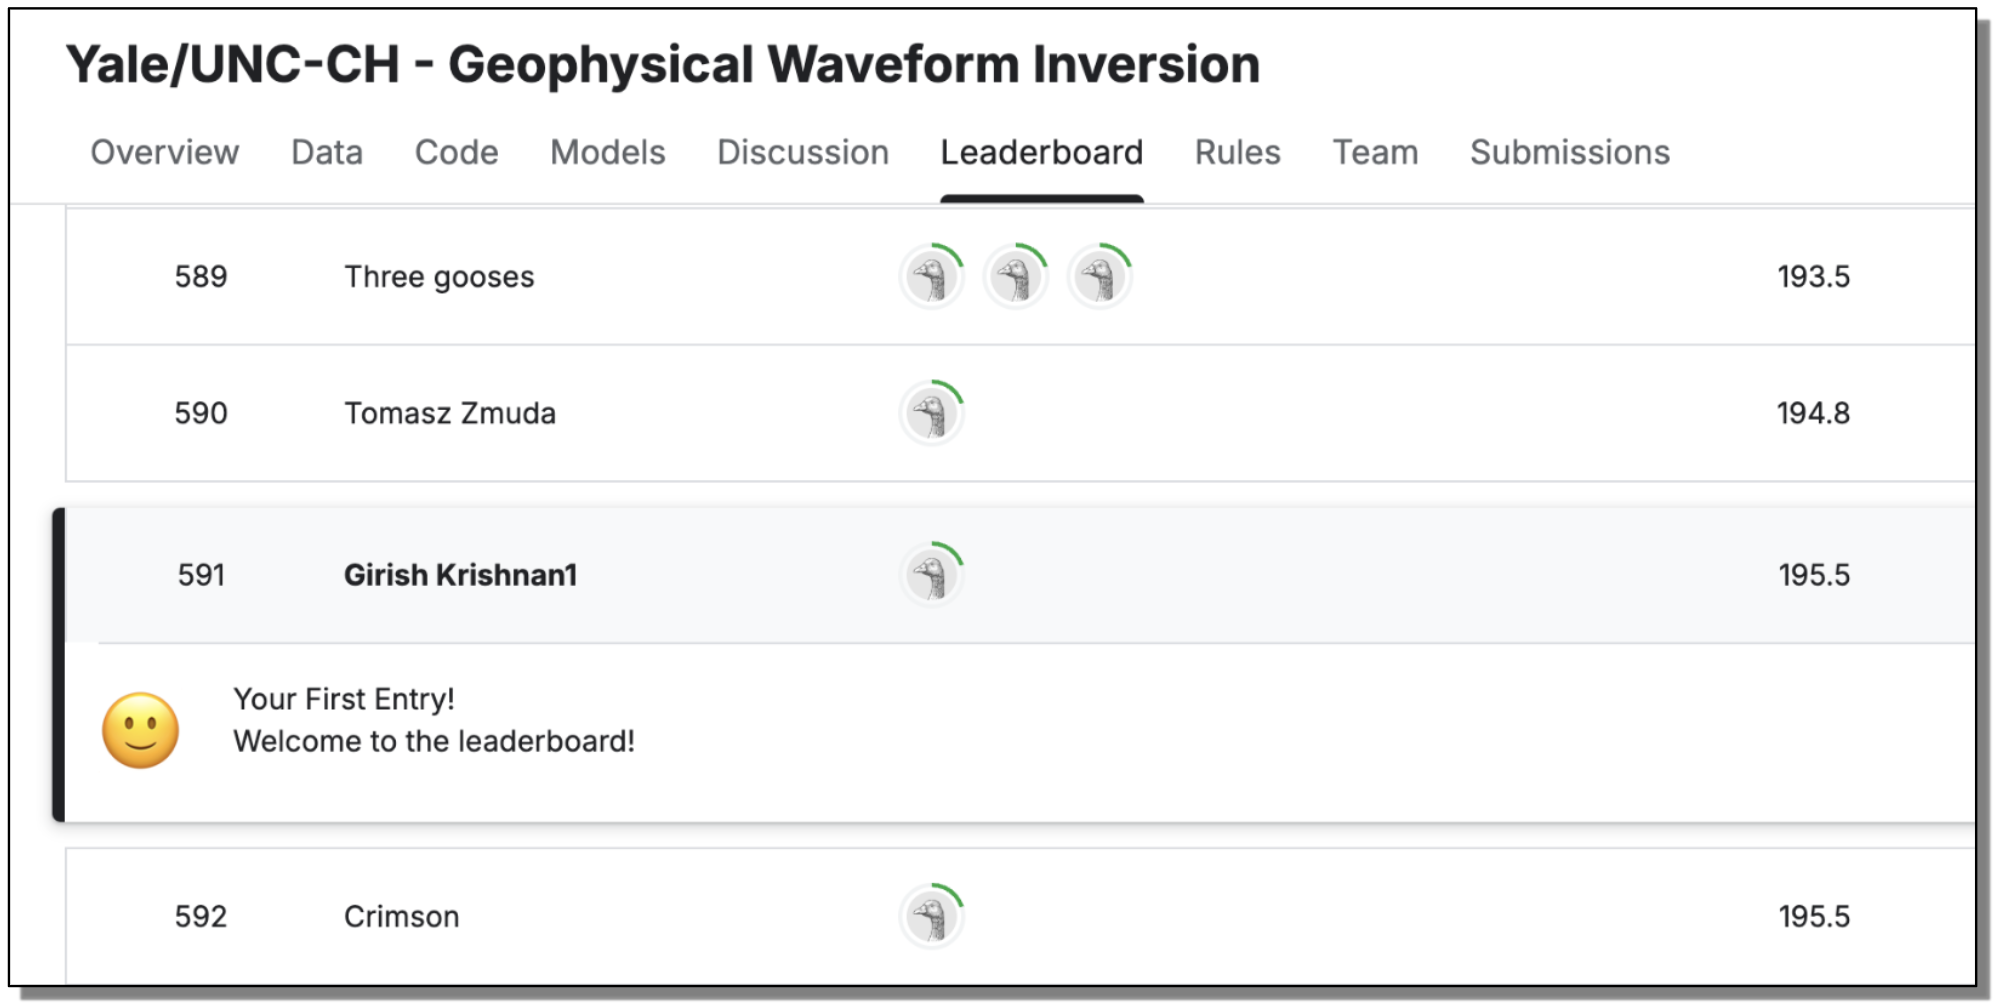
\includegraphics[width=\linewidth]{figures/kaggle_rank.png}
        \caption{Public-leaderboard rank (591/6\,446).}
        \label{fig:kaggle_submission}
    \end{subfigure}
    \hfill
    \begin{subfigure}[b]{0.32\linewidth}
        \centering
        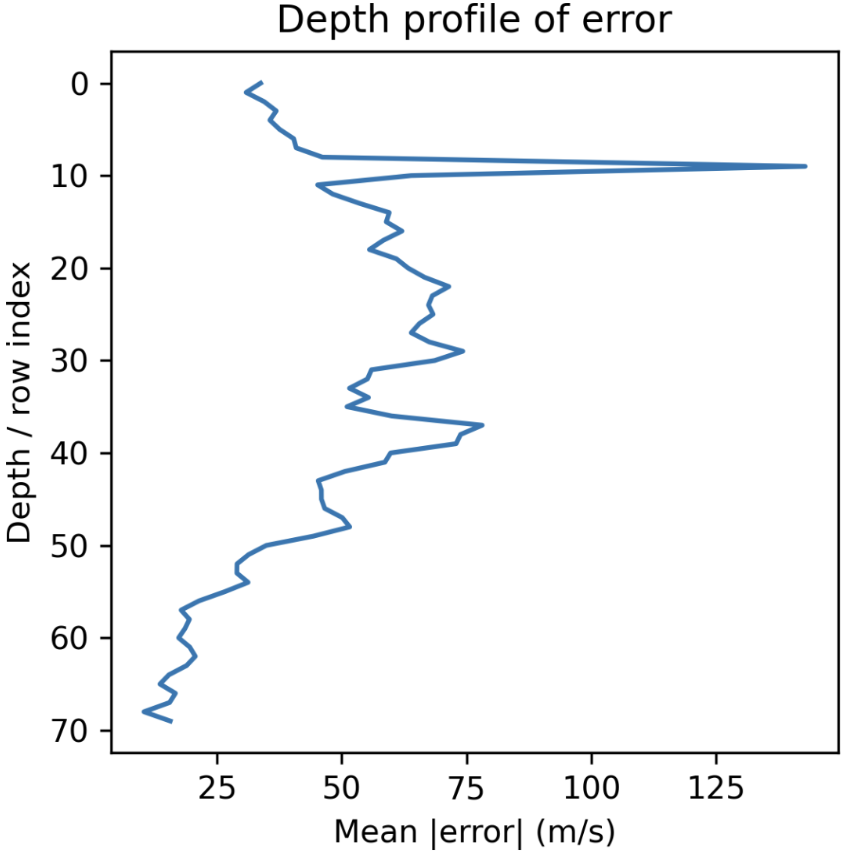
\includegraphics[width=\linewidth]{figures/fdonet_error_depth.png}
        \caption{MAE vs.\ depth.}
        \label{fig:fdonet_depth}
    \end{subfigure}
    \hfill
    \begin{subfigure}[b]{0.32\linewidth}
        \centering
        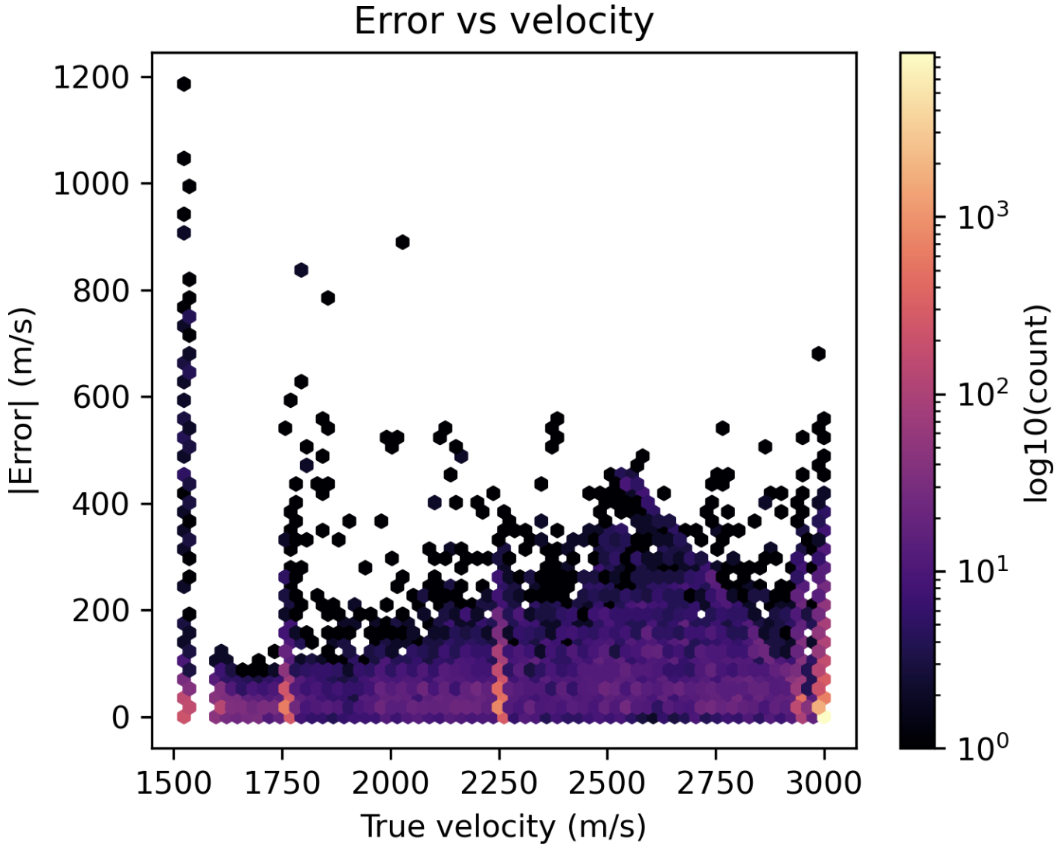
\includegraphics[width=\linewidth]{figures/fdonet_error_velocity.png}
        \caption{MAE vs.\ velocity.}
        \label{fig:fdonet_vel}
    \end{subfigure}
    \vspace{-4pt}
    \caption{Fourier-DeepONet submission analysis on the hidden Kaggle test set. Figure (a) shows our current public leaderboard rank of 591 out of 6,446 participants. Figures (b) and (c) plot the mean absolute error (MAE) of our predictions against depth and velocity, respectively. This gives us insight into how well the model generalizes across different geological scenarios.}
    \label{fig:kaggle_triptych}
\end{figure}

\paragraph{Distributed training protocol.} To reach the 622 GB OpenFWI scale, we trained the best-in-validation \emph{Fourier DeepONet} with \textbf{torchrun} on $2 \times 2080$ GPUs.  
Each GPU processed a \textit{per-device} batch of four shots; gradients were accumulated for one step and synchronized by \textbf{Distributed Data Parallel} (DDP).  Key settings mirror Table~\ref{tab:hparams} but employ \textbf{AdamW} ($\eta =3\times10^{-4}$, weight decay $10^{-4}$), FP16 mixed precision, exponential moving average (EMA, $\alpha=0.999$), and early stopping after 15 stagnant epochs.  

Training converged in $80$ epochs (\(\approx\) 18 GPU-hours).  
The resulting EMA weights were used to generate the competition submission; on the hidden test split Kaggle reports an \textbf{MAE of 195.5\,m/s}.  
The gap with our in-house validation (71.4\,m/s) implies a distribution shift between \textsc{OpenFWI} and the competition data, especially at larger depths and higher velocities (Figure~\ref{fig:kaggle_triptych}b–c), motivating future research on domain adaptation.

\section{Conclusion}
% \instructions{Conclusion [5\%]: Summarize your project and findings. High-level discussion about what you have learned from this project, what works, and what does not work, and ideas/suggestions for future work if you/others want to work on this problem.} 

\subsection{Summary and Key Insights}

This project investigated a variety of data-driven models for seismic-to-velocity inversion. We implemented baseline architectures (InversionNet, VelocityGAN, Residual UNet), advanced neural operators (Fourier DeepONet, FNO), and a PCA-MLP dimensionality reduction pipeline. Among these, the Fourier DeepONet achieved the lowest test error on the Kaggle competition set when trained on the full OpenFWI dataset. Architectures that preserved spatial structure and captured long-range correlations consistently outperformed simpler MLP-based models.

\subsection{What Worked and What Did Not}

Convolutional and operator-based models like UNet, DeepONet, and FNO were the most effective, as they leveraged spatial continuity and hierarchical features. Lightweight models like PCA-MLP were fast but less accurate due to loss of spatial information. Training on the reduced Kaggle subset led to frequent overfitting, indicating the need for larger-scale data or better regularization.

\subsection{Future Directions}

Future work can focus on three areas:
\begin{itemize}[leftmargin=*, itemsep=1pt, topsep=2pt]
    \item \textbf{Noise Robustness:} Evaluate model stability under input perturbations to simulate real-world sensor noise, following findings in \cite{fdonet}.
    \item \textbf{Full-Scale Training:} Extend training of all models to the full OpenFWI dataset. Currently, only the Fourier DeepONet has been fully scaled.
    \item \textbf{Dimensionality Reduction with Stronger Backbones:} Replace the MLP in PCA-MLP with spatially-aware architectures like CNNs. Figure~\ref{fig:conclusion1} illustrates this proposed PCA-CNN pipeline.
\end{itemize}

\begin{figure}[H]
    \centering
    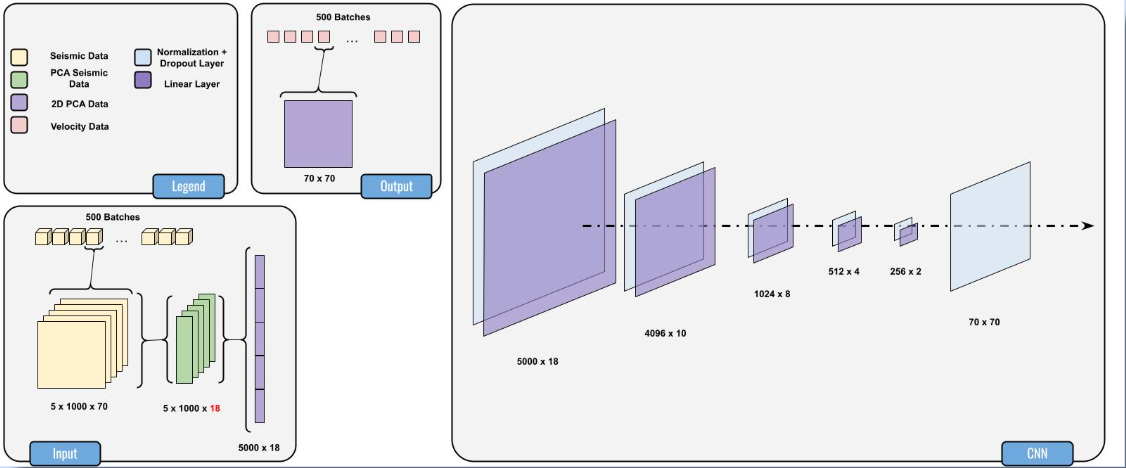
\includegraphics[width=0.8\linewidth]{figures/conclusion1.png}
    \caption{Proposed PCA-CNN architecture combining dimensionality reduction with a convolutional backbone.}
    \label{fig:conclusion1}
\end{figure}

\newpage
% \instructions{The following sections do not count towards the 8-Page Limits.}
\section*{Appendix}
\subsection*{GitHub Link}
% \instructions{Github Link [10\%]. Include a Link to your Project Github with your project codes with necessary documentation. Please include a top-level README.md file in your github repo. This top-level README should explain the layout of this repository and instructions such that users can run your code. Ensure your code can run and reproduce the results you presented in the report. Note that it is your responsibility to ensure that the code repo is working and the README.md is clear to follow.}

The link to our GitHub repository is as follows: \url{https://github.com/Girish-Krishnan/ECE-228-Final-Project/tree/main}. 

This repo contains all the code used to run our models, including the data preprocessing, model training, and evaluation scripts. The \texttt{README.md} file provides detailed instructions on how to set up the environment, install dependencies, and run the code to reproduce our results.

\subsection*{Team Member Contribution}
% \instructions{Describing each team member's contribution for this project (e.g., conceptualization, Data curation, Methodology, Software/Experiments, Report Writing, Poster preparation, etc)} 
Table \ref{tab:team_contrib} summarizes the contributions of each team member to the project. The goal was to have each team member implement at least 1-2 different model architectures so that we have several different models to compare against each other. The team members were also responsible for writing the report and poster sections that corresponded to their model implementations.

\begin{table}[H]
    \centering
    \renewcommand{\arraystretch}{1.4}
    \setlist[itemize]{leftmargin=1.5em, topsep=2pt, itemsep=1pt}
    \begin{tabular}{p{3.5cm} p{11cm}}
        \toprule
        \textbf{Member} & \textbf{Key Contributions} \\
        \midrule

        \textbf{Harini Gurusankar} &
        \begin{itemize}
            \item Designed the baseline \emph{Neural ODE} and \emph{Augmented Neural ODE} models.
            \item Implemented MLP and CNN-based ODE variants in PyTorch.
            \item Wrote the methodology subsection and results discussion for ODE models.
            \item Contributed methodology content to the poster and presented it.
        \end{itemize} \\

        \textbf{Girish Krishnan} &
        \begin{itemize}
            \item Coordinated the project and designed the experimental pipeline.
            \item Implemented \emph{Fourier DeepONet}, residual \emph{UNet}, \emph{InversionNet}, and \emph{VelocityGAN}.
            \item Trained and submitted full-data DeepONet (best MAE: 59.5 m/s).
            \item Created metric visualizations (bar charts, heatmaps, radar plots).
            \item Wrote the abstract and results sections.
            \item Designed and presented the results section of the poster.
        \end{itemize} \\

        \textbf{Ryan Irwandy} &
        \begin{itemize}
            \item Developed the PCA-based baseline and accompanying MLP model.
            \item Wrote PCA utilities and normalization scripts.
            \item Ran experiments on component counts and dropout strategies.
            \item Wrote parts of the related work and methodology sections.
            \item Created and presented the poster’s introduction and PCA baseline sections.
        \end{itemize} \\

        \textbf{Yash Puneet} &
        \begin{itemize}
            \item Implemented the 2-D \emph{Fourier Neural Operator} with spectral blocks.
            \item Tuned mode counts and channel widths via hyperparameter sweeps.
            \item Created architecture figures for the FNO section.
            \item Wrote FNO-related work, methodology, and future work sections.
            \item Designed and presented the related work and future work sections of the poster.
        \end{itemize} \\

        \bottomrule
    \end{tabular}
    \caption{Summary of individual contributions to the project.}
    \label{tab:team_contrib}
\end{table}


\subsection*{Confirmation of Teaching Evaluation Submission}

Our team confirms that we have submitted our teaching evaluation for the ECE 228 course and the teaching assistant evaluations. Here are screenshots that confirm our submission:

\begin{figure}[H]
    \centering
    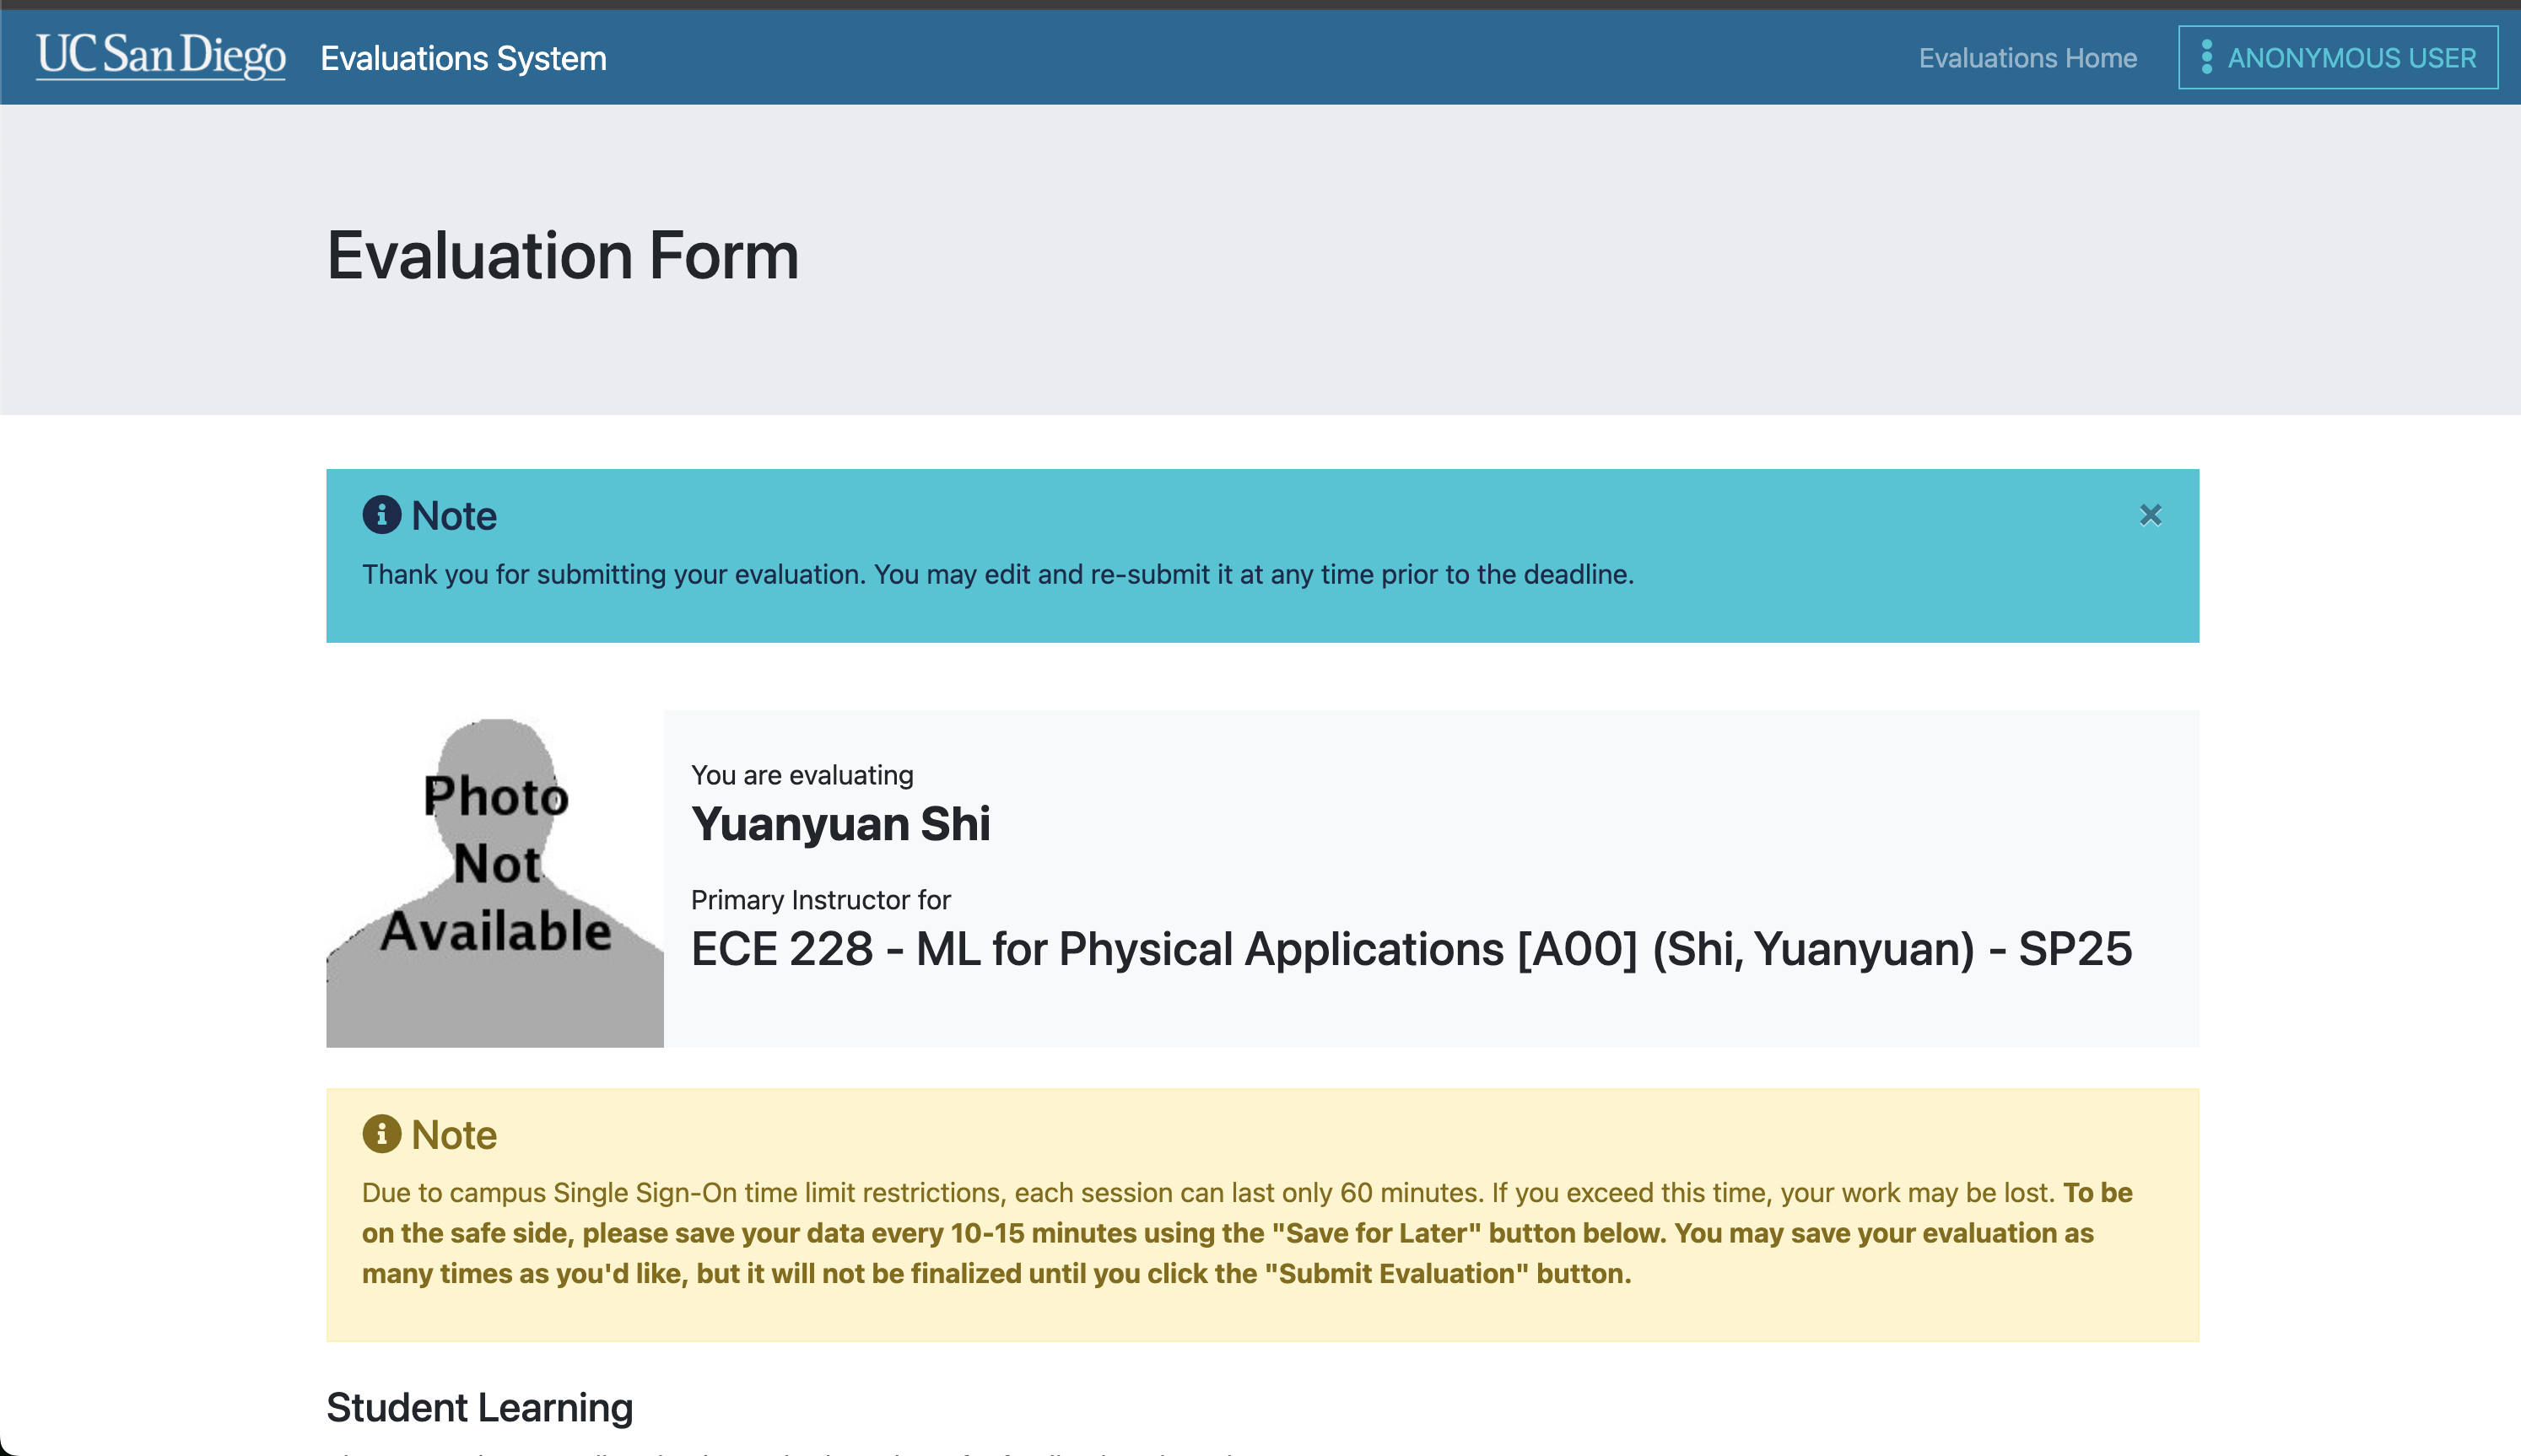
\includegraphics[width=0.49\linewidth]{figures/teaching_evaluations/instructor_eval.png}
    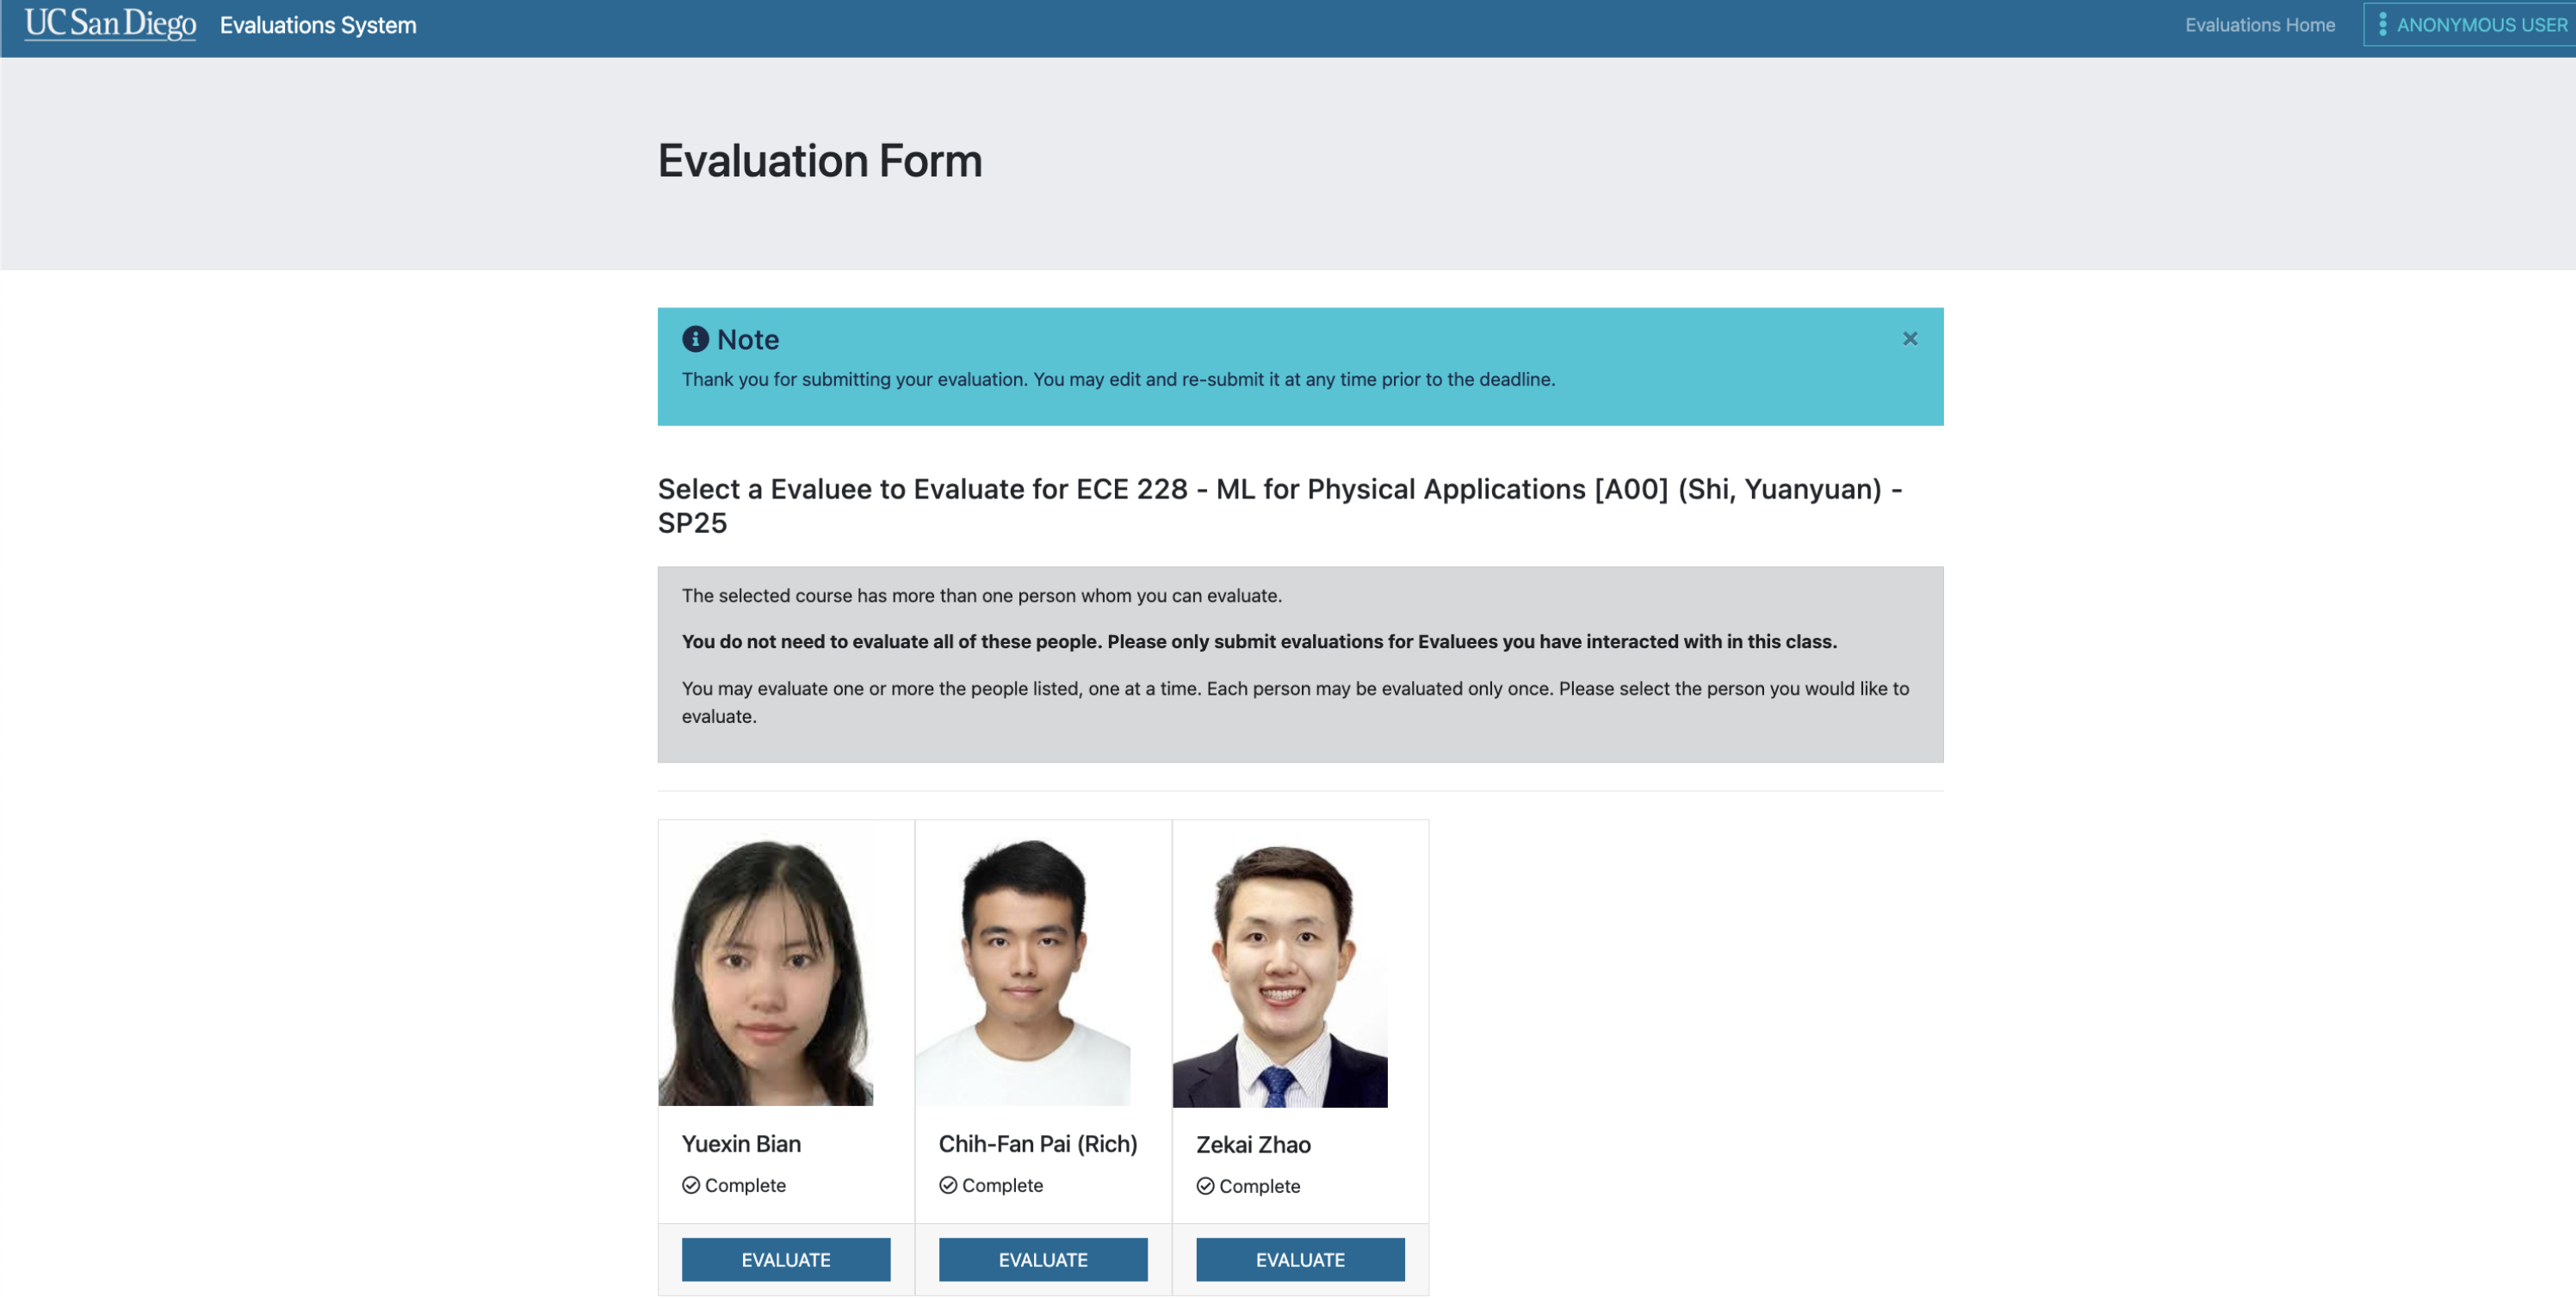
\includegraphics[width=0.49\linewidth]{figures/teaching_evaluations/ta_eval.png}
    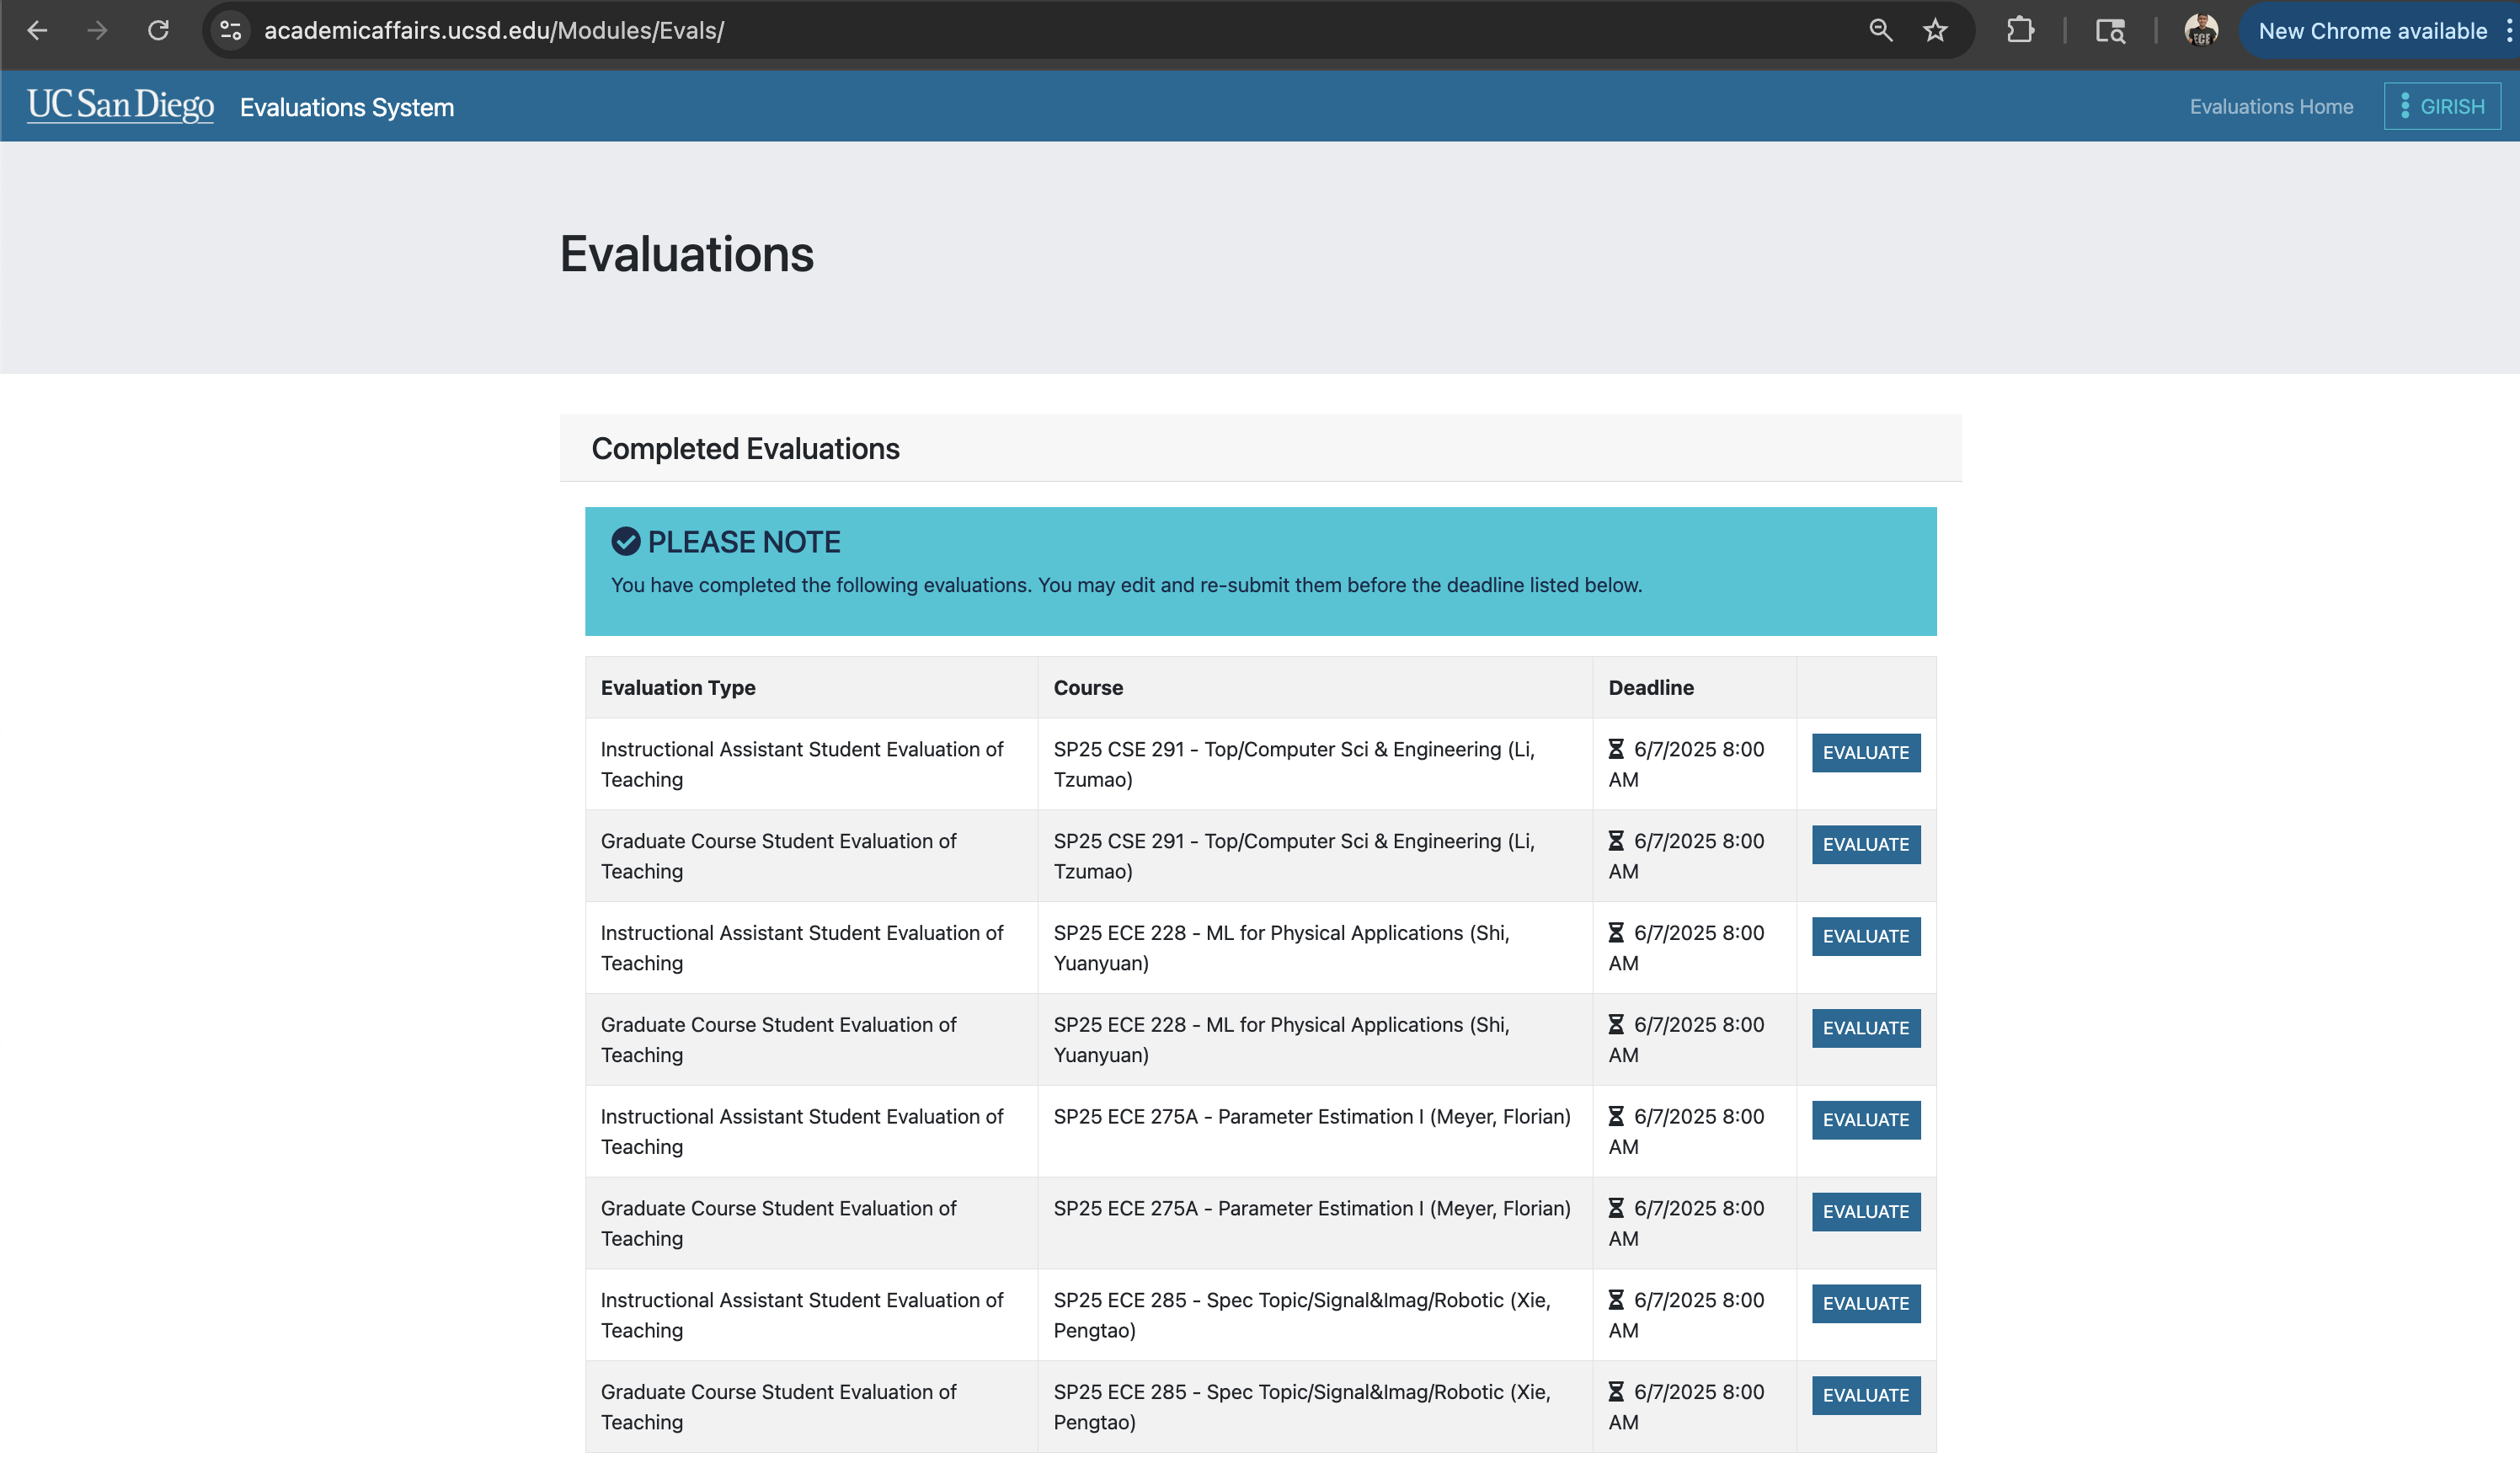
\includegraphics[width=\linewidth]{figures/teaching_evaluations/set_eval.png}
    \caption{Teaching Evaluation Submission Confirmation}
    \label{fig:teaching_evaluation}
\end{figure}

Thanks for teaching us this awesome course!


\bibliography{bib}
\bibliographystyle{abbrvnat}








\end{document}
